\chapter{Antena Escollida}

Vistes les anàlisis anteriors, a l'hora d'escollir entre una antena monopol i una antena dipol per a la seva construcció, s'ha escollit la segona opció, és a dir, la \textbf{construcció d'una antena monopol}.

S'ha escollit aquesta antena doncs s’ha cregut més pràctica i amb més potenciala degut principalment al fet que permet una possible futura expansió cap a una antena Yagi per tal de fer-la més directiva. 

Per altra banda, una antena monopol tindrà una impedància d’entrada de 36 $\si{\ohm}$ en el millor dels casos. Per tant la desadaptació amb un cable de 75 $\si{\ohm}$ serà força gran. Inclús amb un cable de 50 serà superior a la que tindria una antena dipol amb 73 $\si{\ohm}$ d’impedància amb un cable de 75 $\si{\ohm}$.

Així doncs, per una freqüència central de treball de 122 MHz:

\begin{equation}
\notag
  \lambda=\frac{c}{f}=\frac{3\cdot10^8}{122\cdot10^6}= 2.459\,\mathrm{m}
\end{equation}

Buscant que l'impedància d'entrada no tingui cap part complexa es troba la longitud d'antena L. 

\begin{equation}
\notag
  L=\frac{\lambda}{2}-3\%= 1.156\,\mathrm{m}
\end{equation}

L'antena dipol que serà doncs construida es mostra a la figura \ref{LAntena}.
\begin{figure}[H]
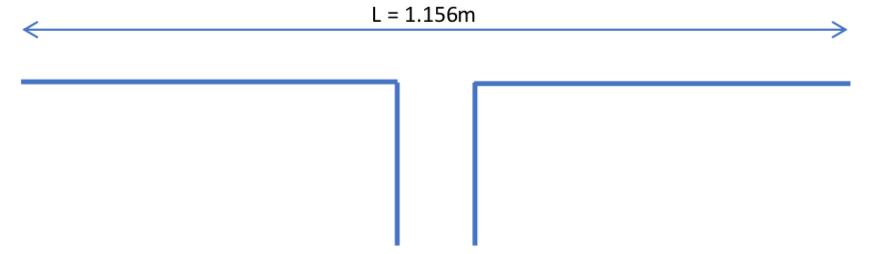
\includegraphics[width=1\textwidth]{./images/LAntena}
\caption{Longitud de l'antena dipol a construir}
\label{LAntena}
\end{figure}

\section{Resistència aerodinàmica paràsita}
Abans de procedir a la construcció de l'antena, es fa un anàlisis aerodinàmic amb \textit{CFD} per tal de determinar el drag paràsit que genera aquesta antena en l'aeronau escollida en condicions de vol.

Les condicions de vol escollides són\footnote{les variables termodinàmiques s'han obtingut amb l'alçada i emprant el model atmosfèric ISA.}:
\begin{itemize}
\item v = 102.9 m/s
\item h = 2400 m
\item T = 272.6 K
\item P = 75625.7 Pa
\item $\rho$ = 0.97
\end{itemize}

El primer pas ha sigut modelar l'antena en \textit{SolidWorks} amb les dimensions determinades prèviament. La malla obtinguda d'aquest model s'observa a les figures \ref{malla1} i \ref{malla2}.

Finalment, amb \textit{\textbf{OpenFoam}} s'han realitzat una sèrie de simulacions a partir de la malla mostrada. Així, s'han obtingut els valors mostrats a la taula \ref{C_opti2}\footnote{El cas d'aeronau comercial empra 8000m d'alçada i un Mach de 0.9.}:
\begin{table}[H]
	\centering
	\begin{tabular}{lc}
		\toprule[3pt]
		\textbf{Cas}&\textbf{$C_d$}\\
		\midrule[1pt]
		Cas de disseny & 0.29 \\
		Cas d'aeronau comercial & 0.14 \\
		\bottomrule[2pt]
	\end{tabular}
	\caption{Drag paràsit del dipol}
	\label{C_opti2}
\end{table}
\begin{figure}[H]
	\centering
	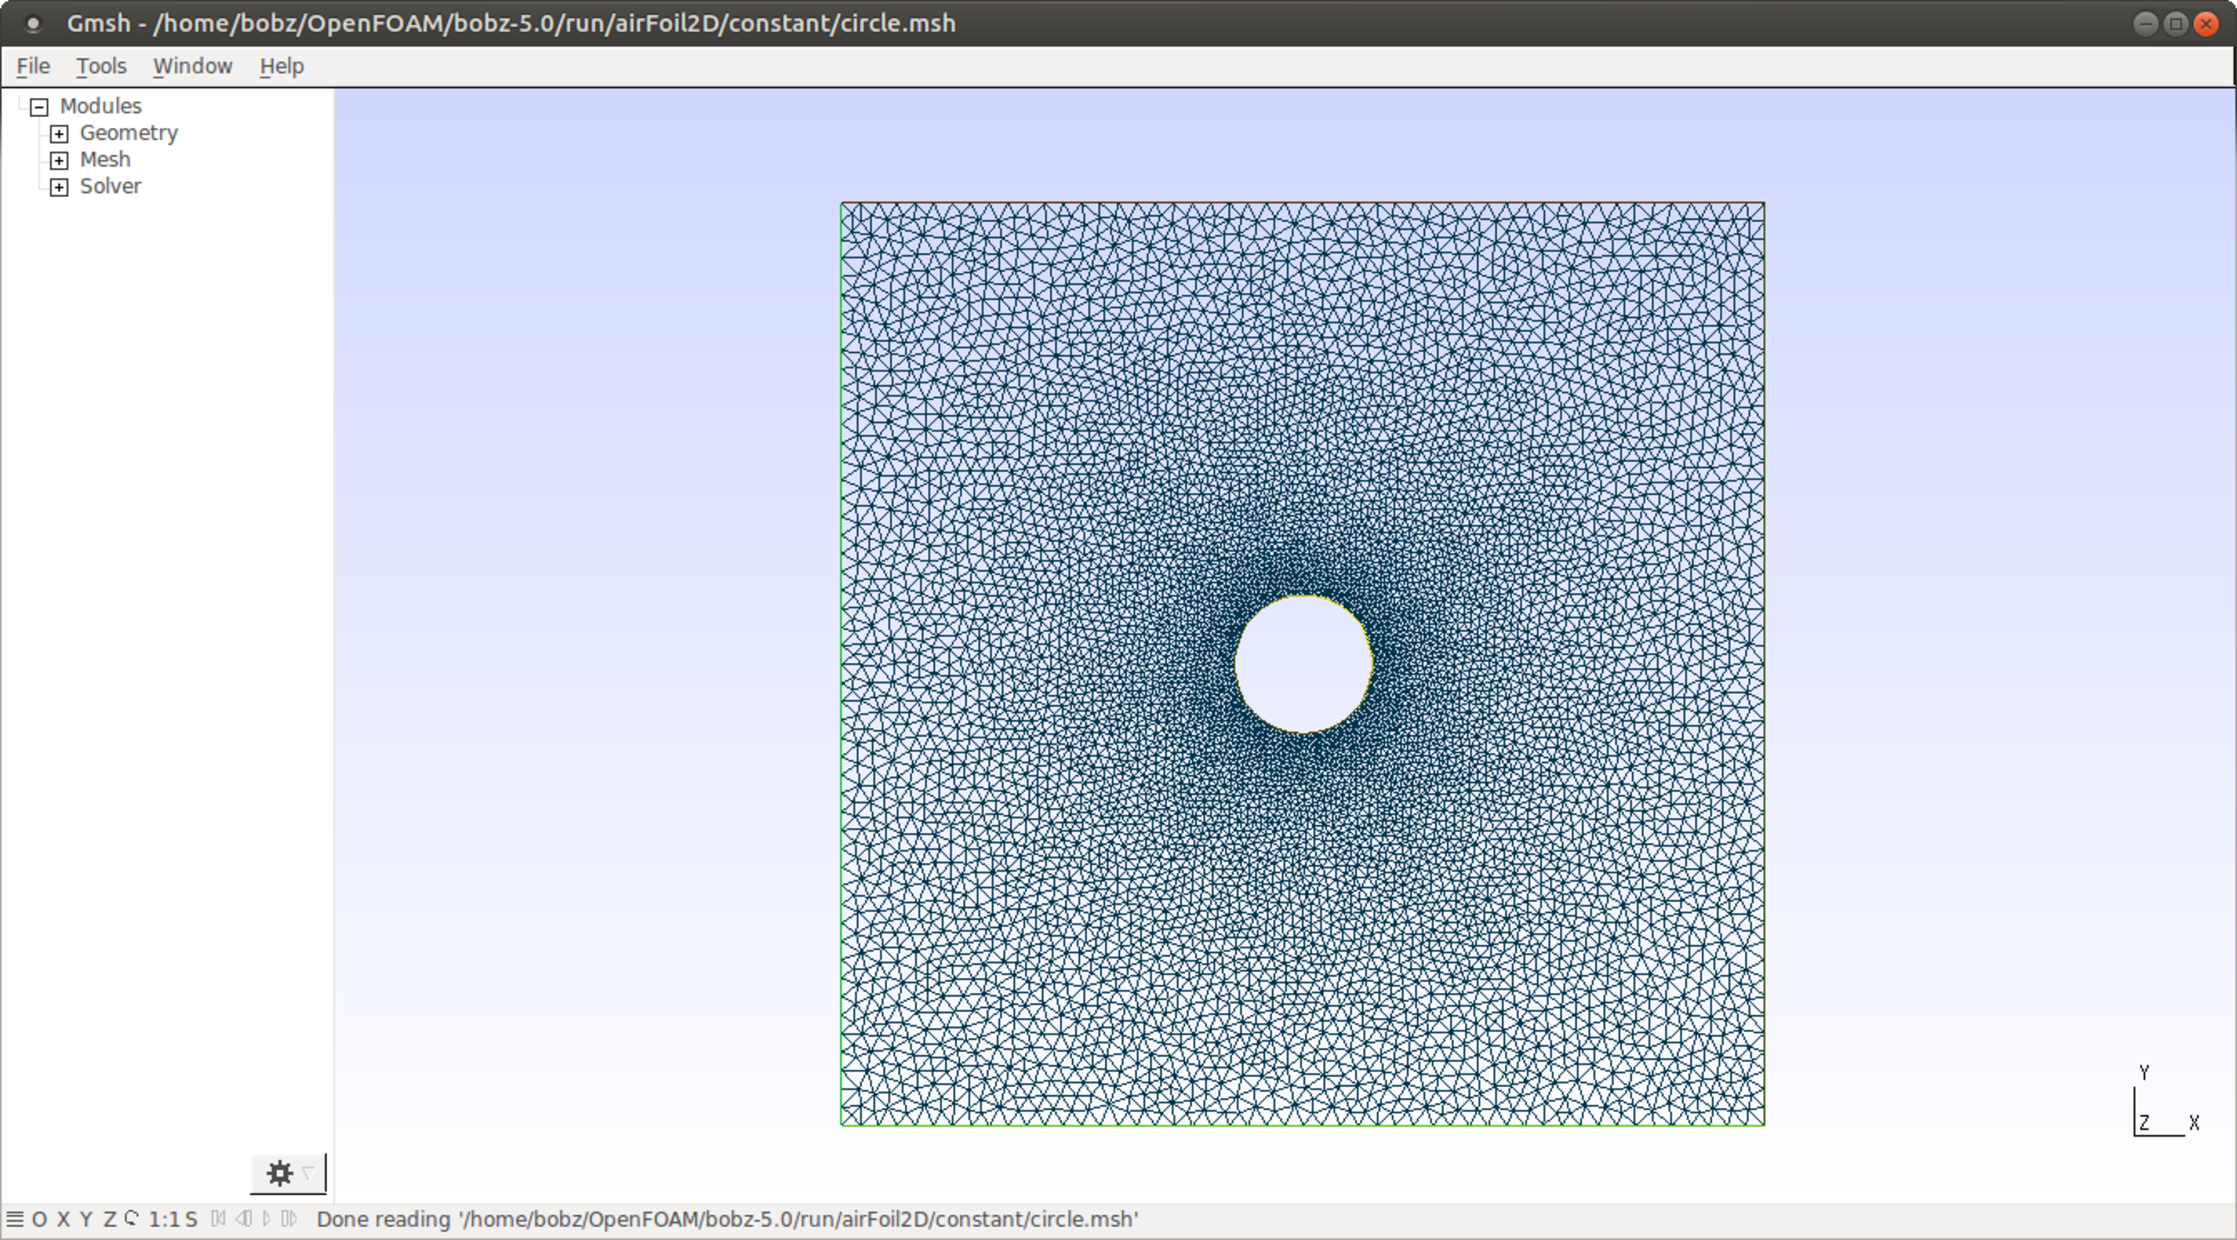
\includegraphics[width=\textwidth]{./images/malla1.pdf}
	\caption{Visió Frontal malla}
	\label{malla1}
\end{figure}
\begin{figure}[H]
	\centering
	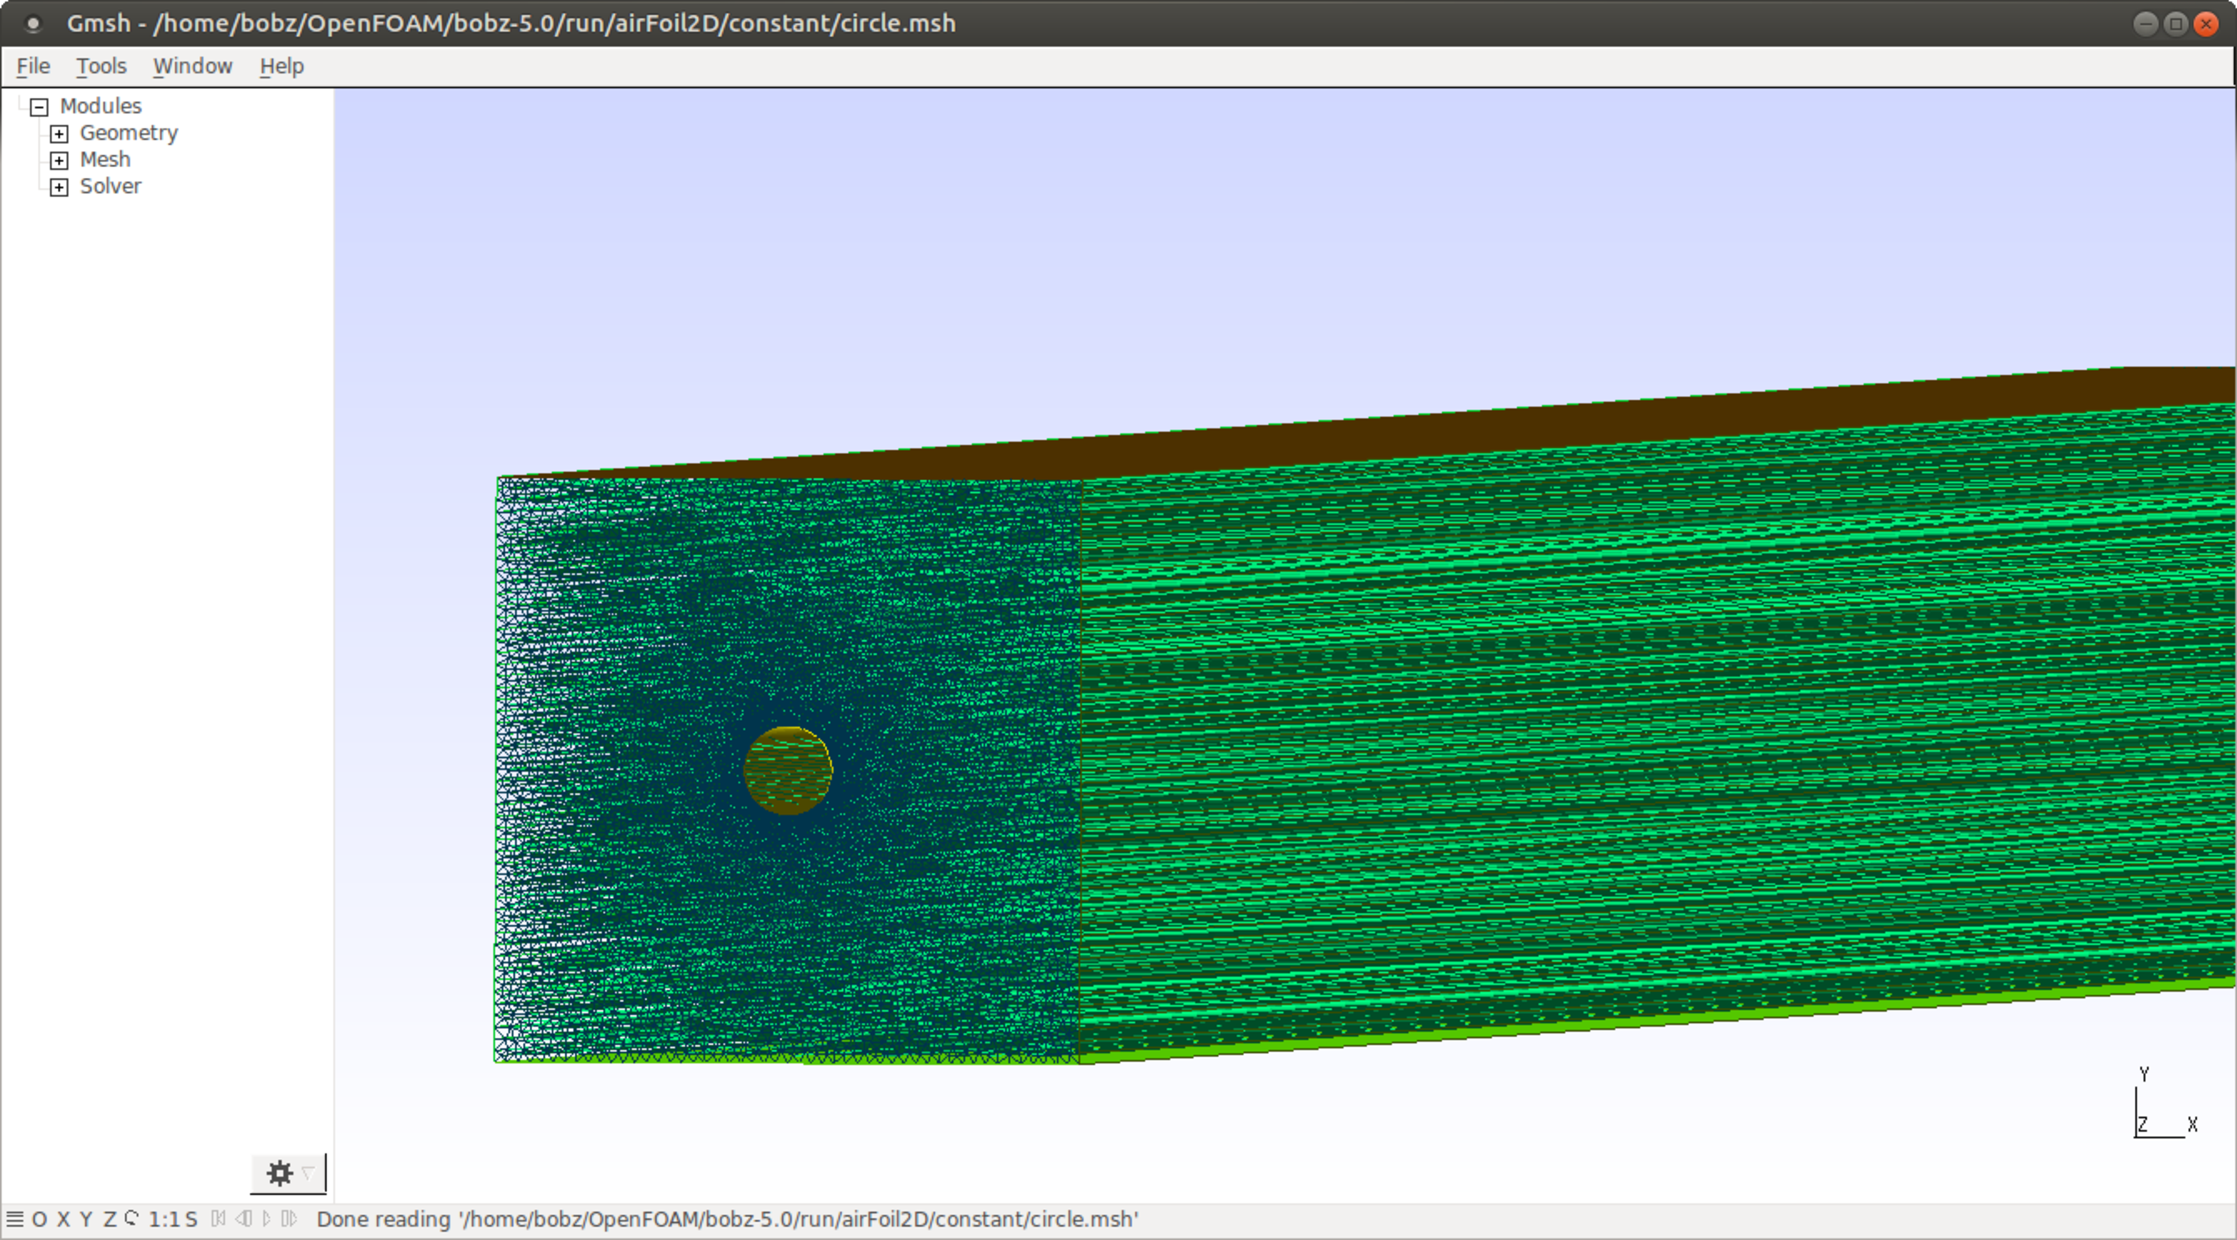
\includegraphics[width=\textwidth]{./images/malla2.pdf}
	\caption{Visió de la malla en perspectiva}
	\label{malla2}
\end{figure}
El forat cilíndric dins del volum de control representa l'antena, i així s'ha especificat a OpenFoam.
\section{Construcció de l'Antena}

La construcció de l'antena dipol considerada consta de dues parts: el desenvolupament del (NO ME ACUERDO COMO SE LLAMA) i la construcció del cap de l'antena.

Cal mencionar que per a realitzar la construcció de l'antena, el parametre més important considerat a estat que fos el més "low cost" possible sense comprometre la funcionalitat.

\textbf{NO ME ACUERDO COMO SE LLAMA}

\textbf{Cap de l'antena}

Per a la construcció del cap de l'antena s'ha utilitzat filferro de 1.5 mm de diàmetre així com una regleta per conectar els dos braços al camble d'alimentació.

A més, per tal de protegir les conexions, aquestes s'han dut a terme dins d'un tupper com es pot veure a la figure %\ref{capAntena} 

((FALTA FOTO DE ANTENA DONDE SE VEAN LAS CONEXIONES))


\textbf{Antena Construida}

Finalment l'antena construida es la mostrada a la figura X %ref{AntenaFinal}

(PONER FOTO FINAL DE LA ANTENA)
\section{Mesures}

Al laboratori es desponia dels següents aparells:
\begin{itemize}
\item \textbf{Network Analyzer}: HP 8752A
\item \textbf{Spectrum Analyzer}: Anritsu MS2601B
\item Adaptdors de cables. S'ha emprat el de tipus IEC a tipus BNC.
\end{itemize}

Així mateix, es va comptar amb el suport del professor de l'assignatura, el Dr. Antoni Barlabé, a qui agraïm la seva disposició.

\begin{figure}[H]
\centering
\begin{subfigure}{.5\textwidth}
	\centering
	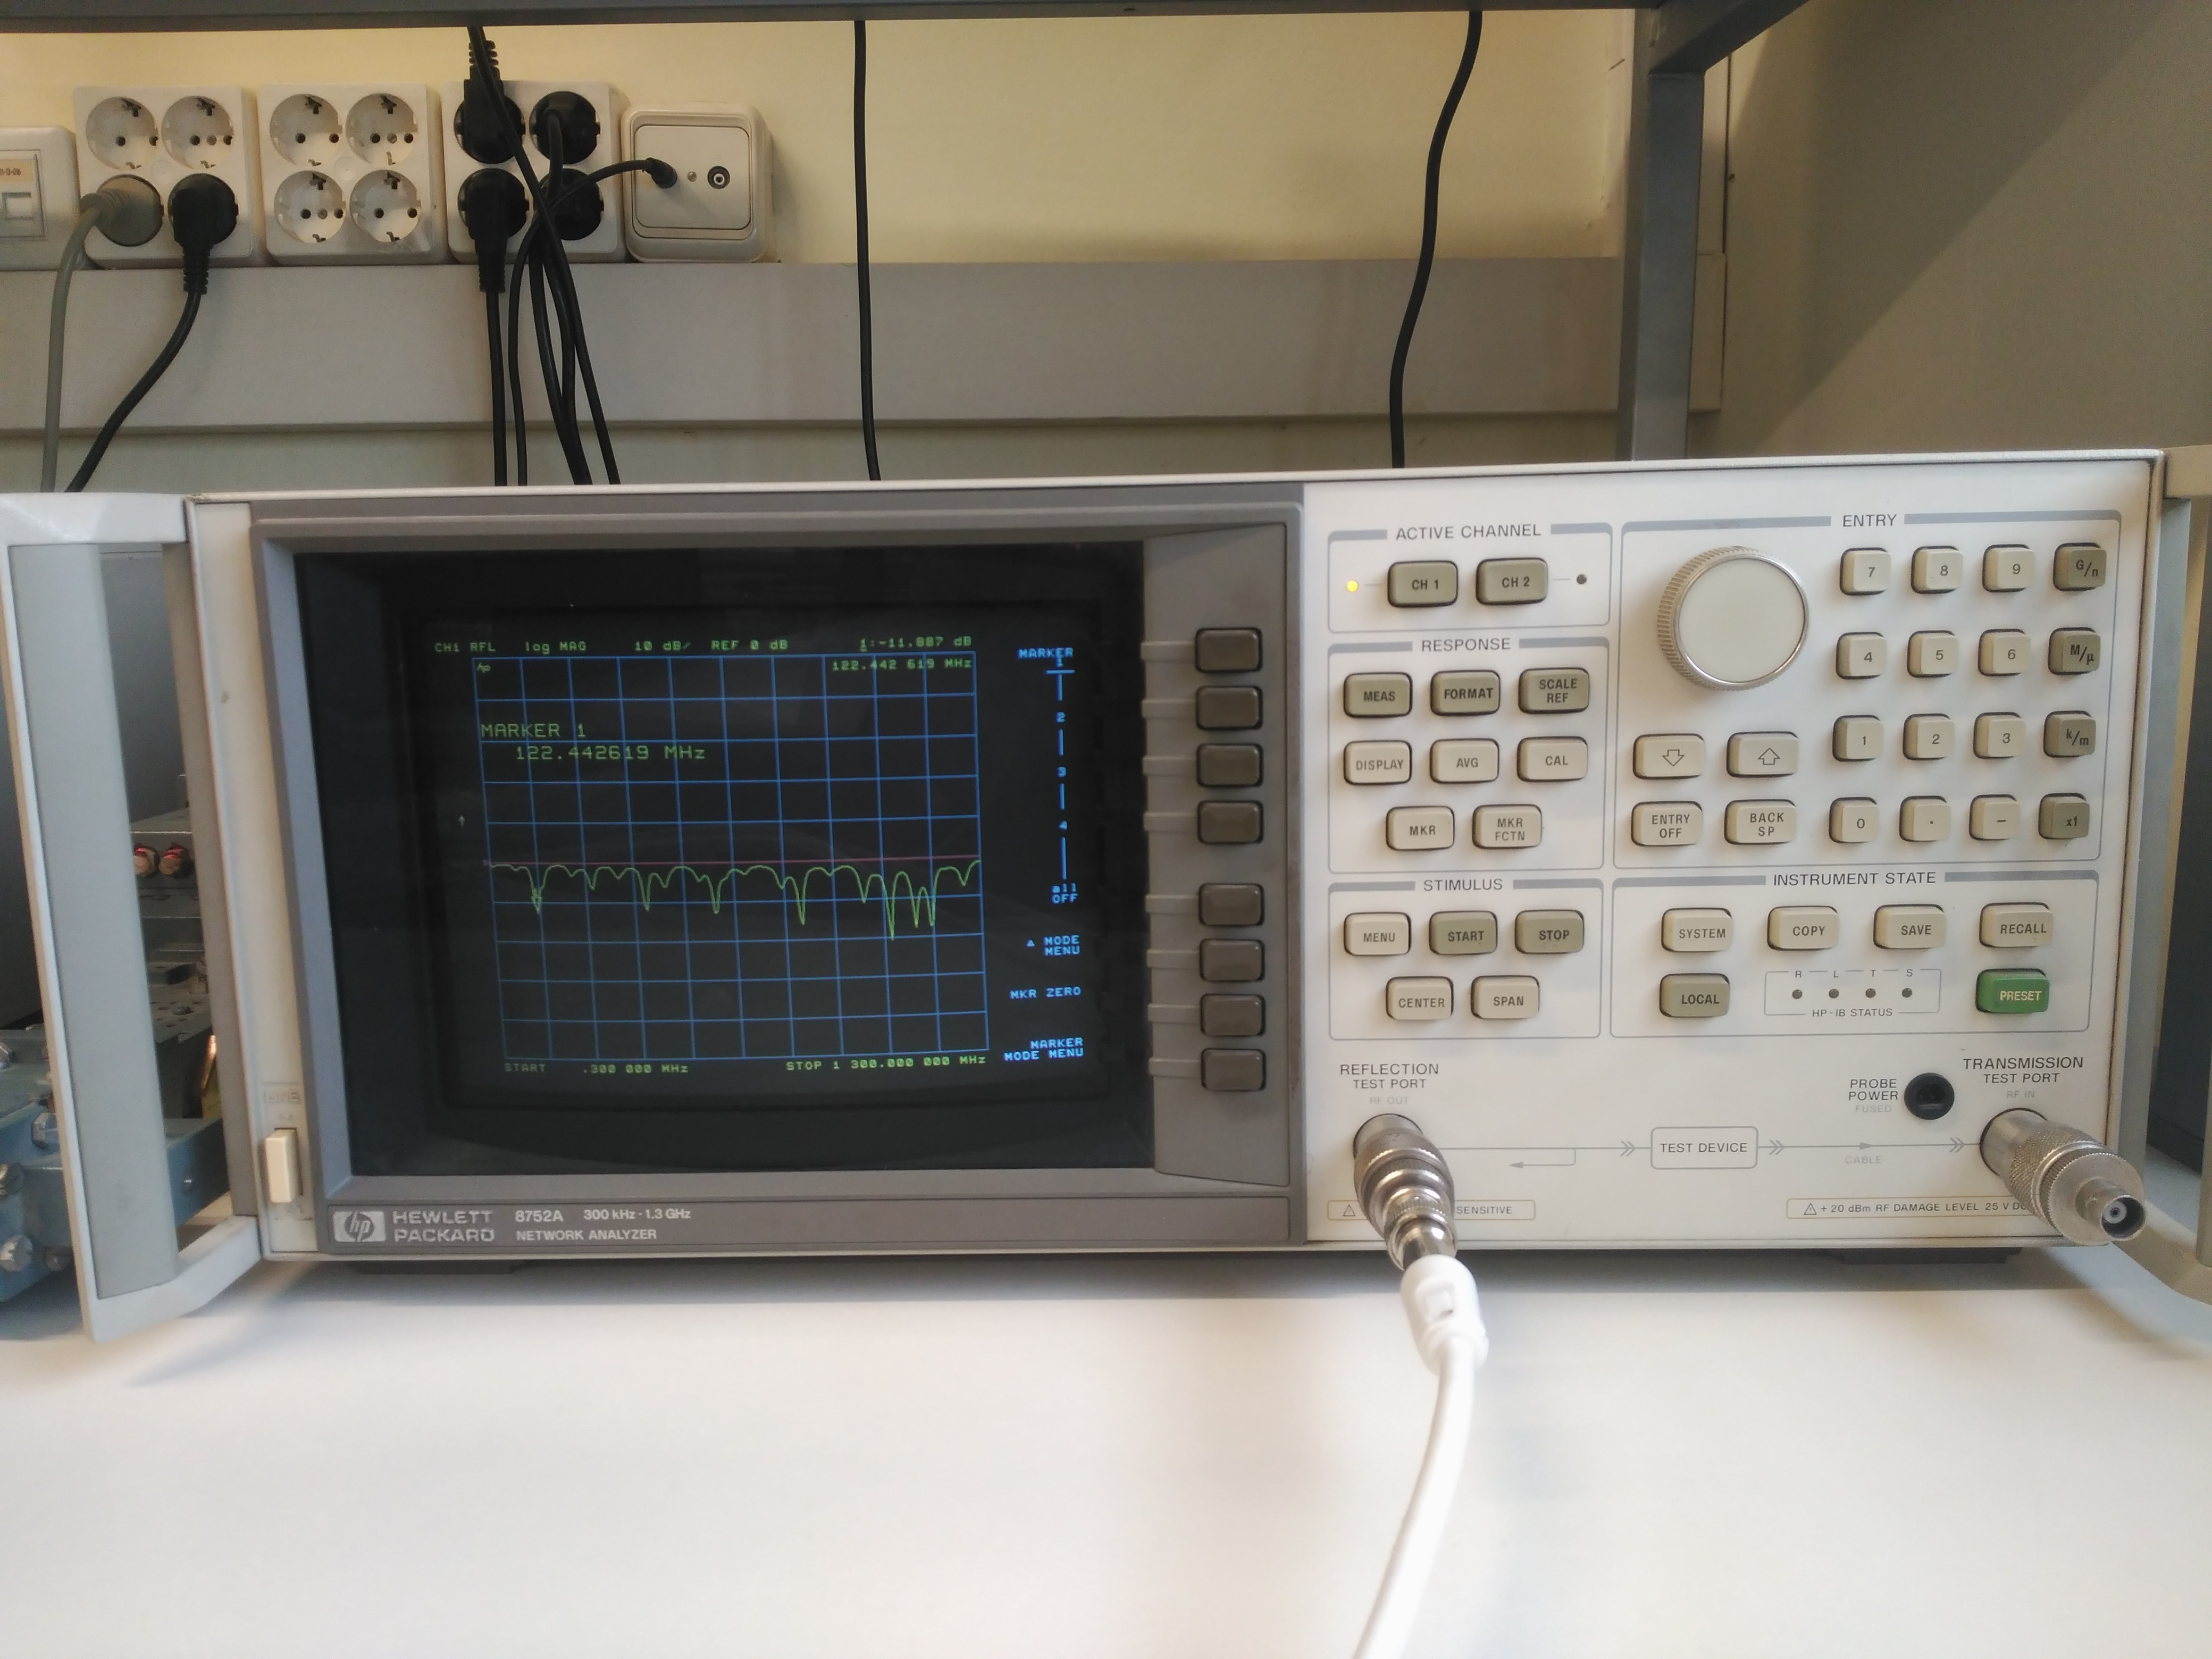
\includegraphics[width=0.9\textwidth]{./images/Mesures/01setUp.jpg}
	\caption{}
	\label{setup1}
\end{subfigure}%
\begin{subfigure}{.5\textwidth}
	\centering
	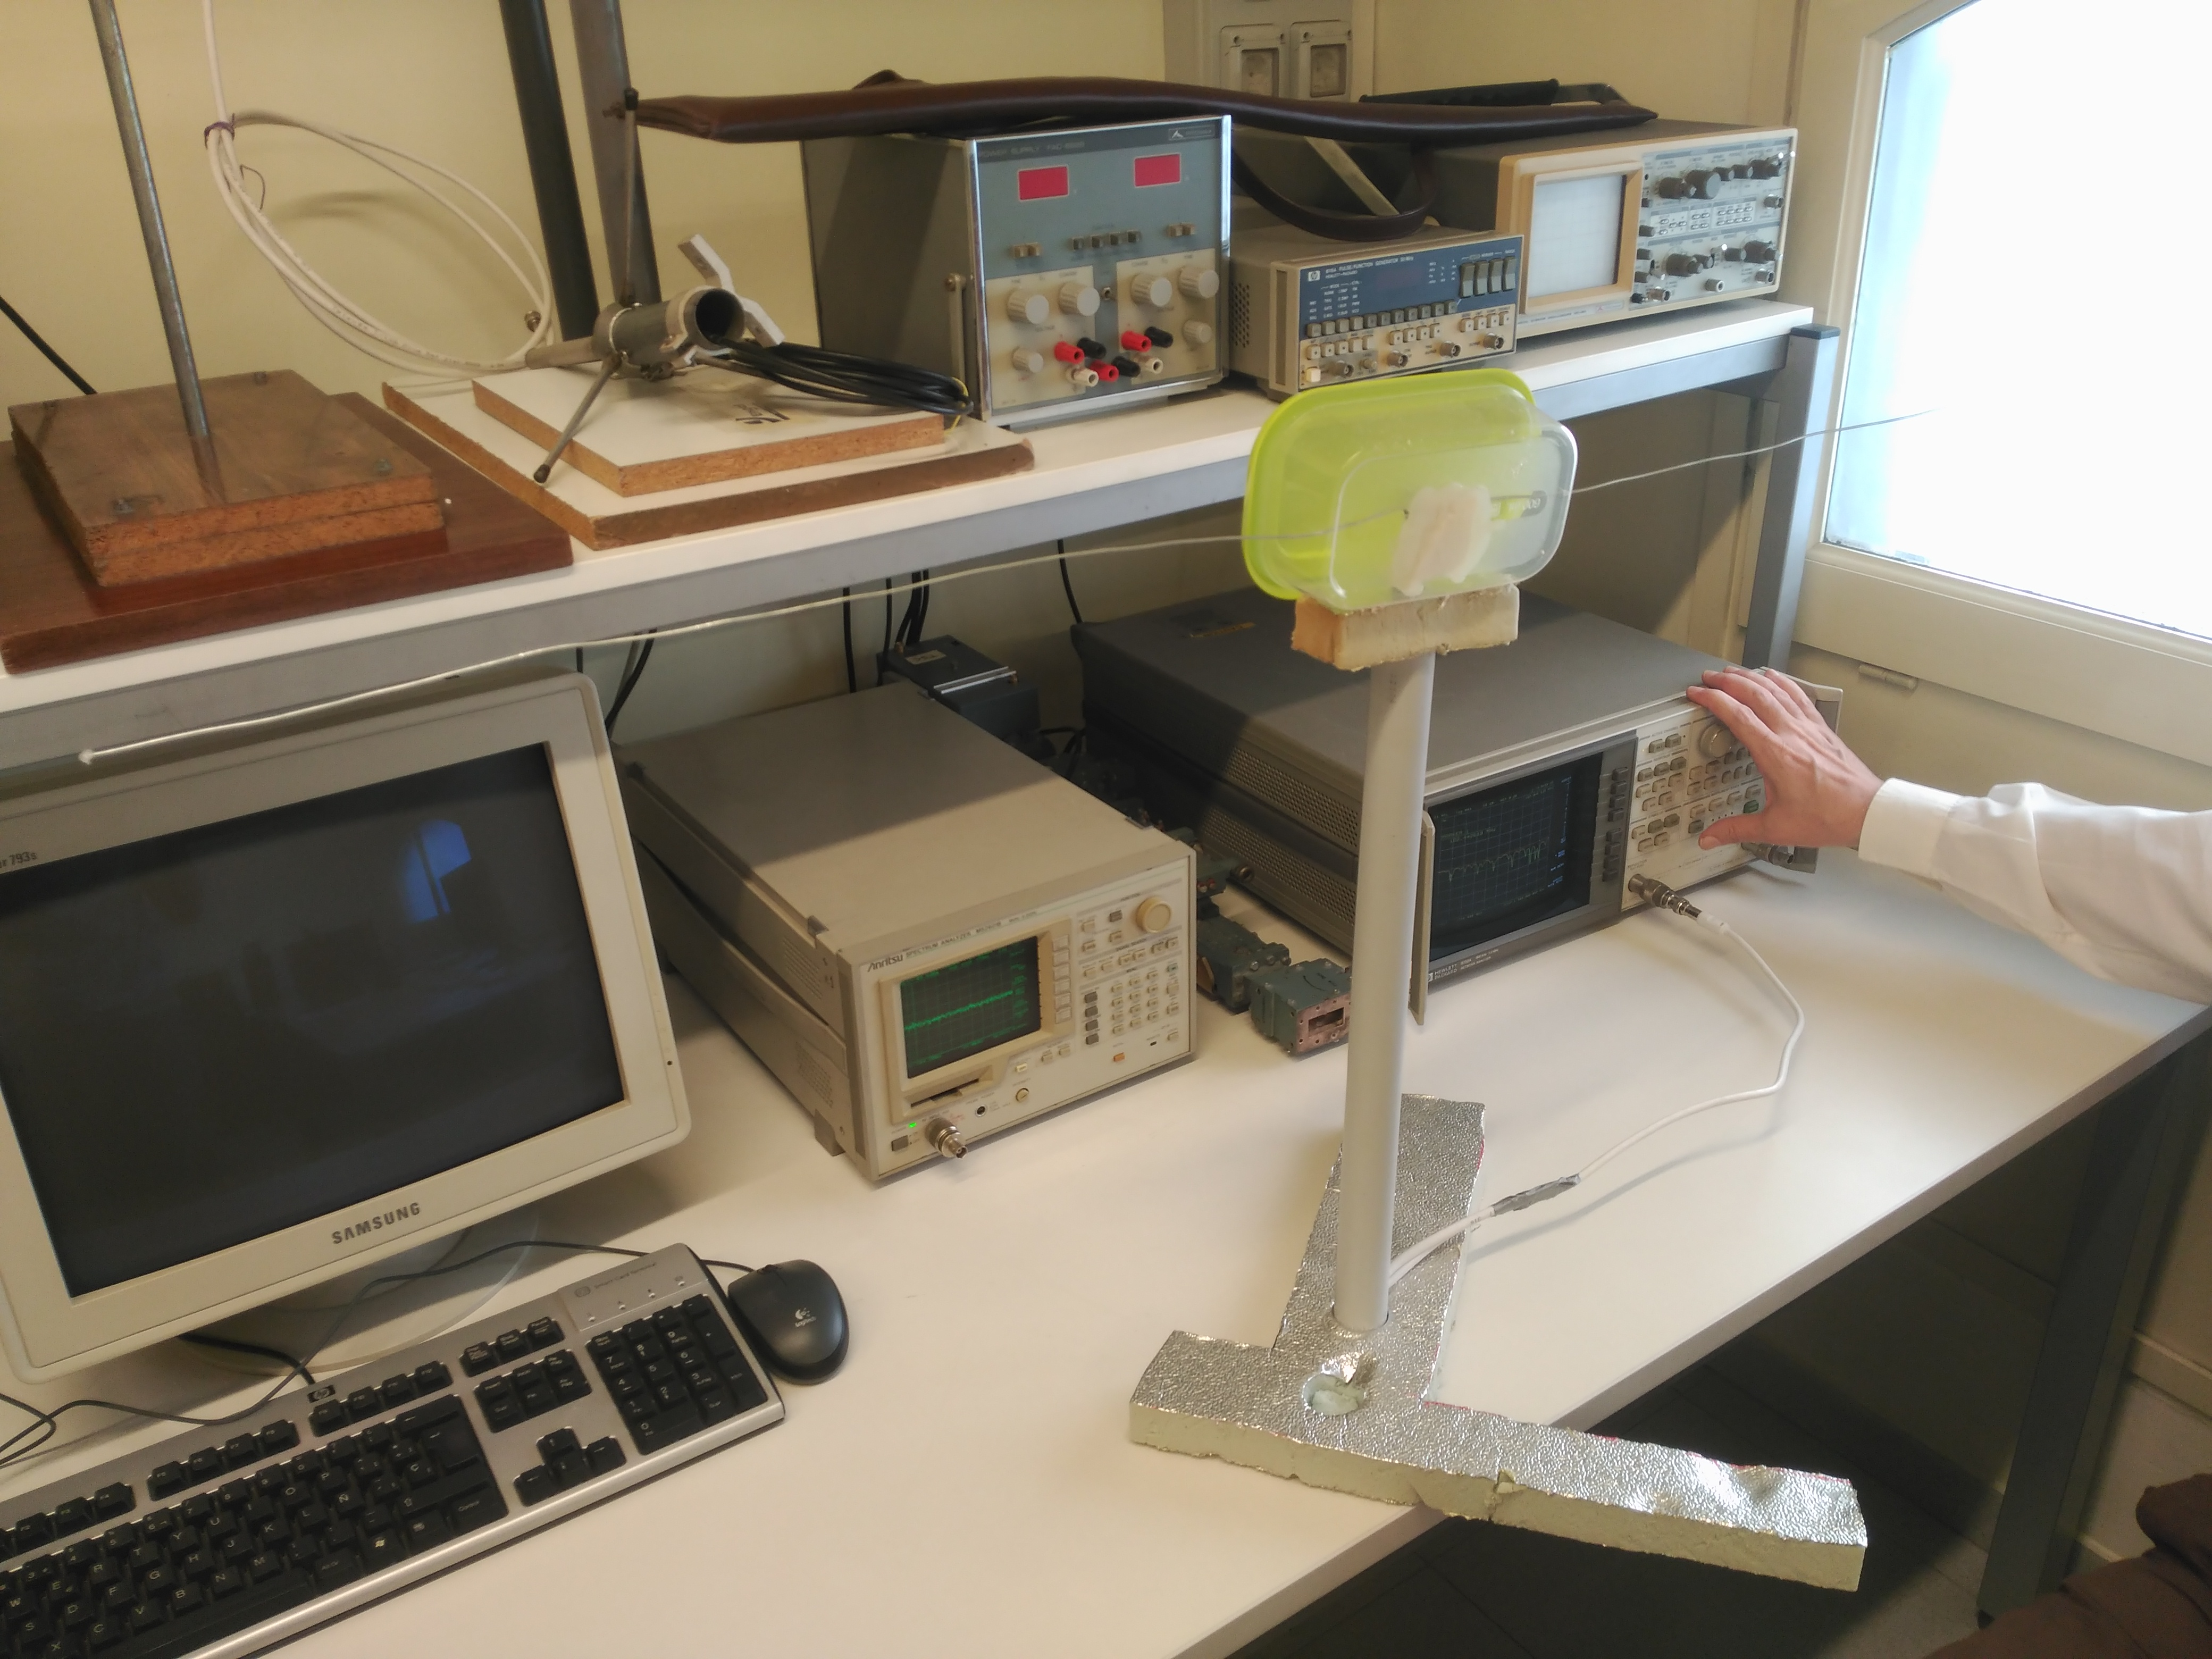
\includegraphics[width=0.9\textwidth]{./images/Mesures/0setUp.jpg}
	\caption{}
	\label{setup2}
\end{subfigure}
\caption{Context del laboratori}
\label{setup}
\end{figure}

\subsection{Mesura del coeficient de reflexió $\Gamma$}
Amb l'analitzador de xarxes vectorial connectat al conjunt antena-connectors-cable-balun, primerament es troba el coeficient de reflexió a l'entrada d'aquest. És recorda:
\begin{equation}
\Gamma = \frac{E_{reflectida}}{E_{emesa}} =\frac{E^-}{E^+}
\end{equation}
\begin{figure}[H]
	\centering
	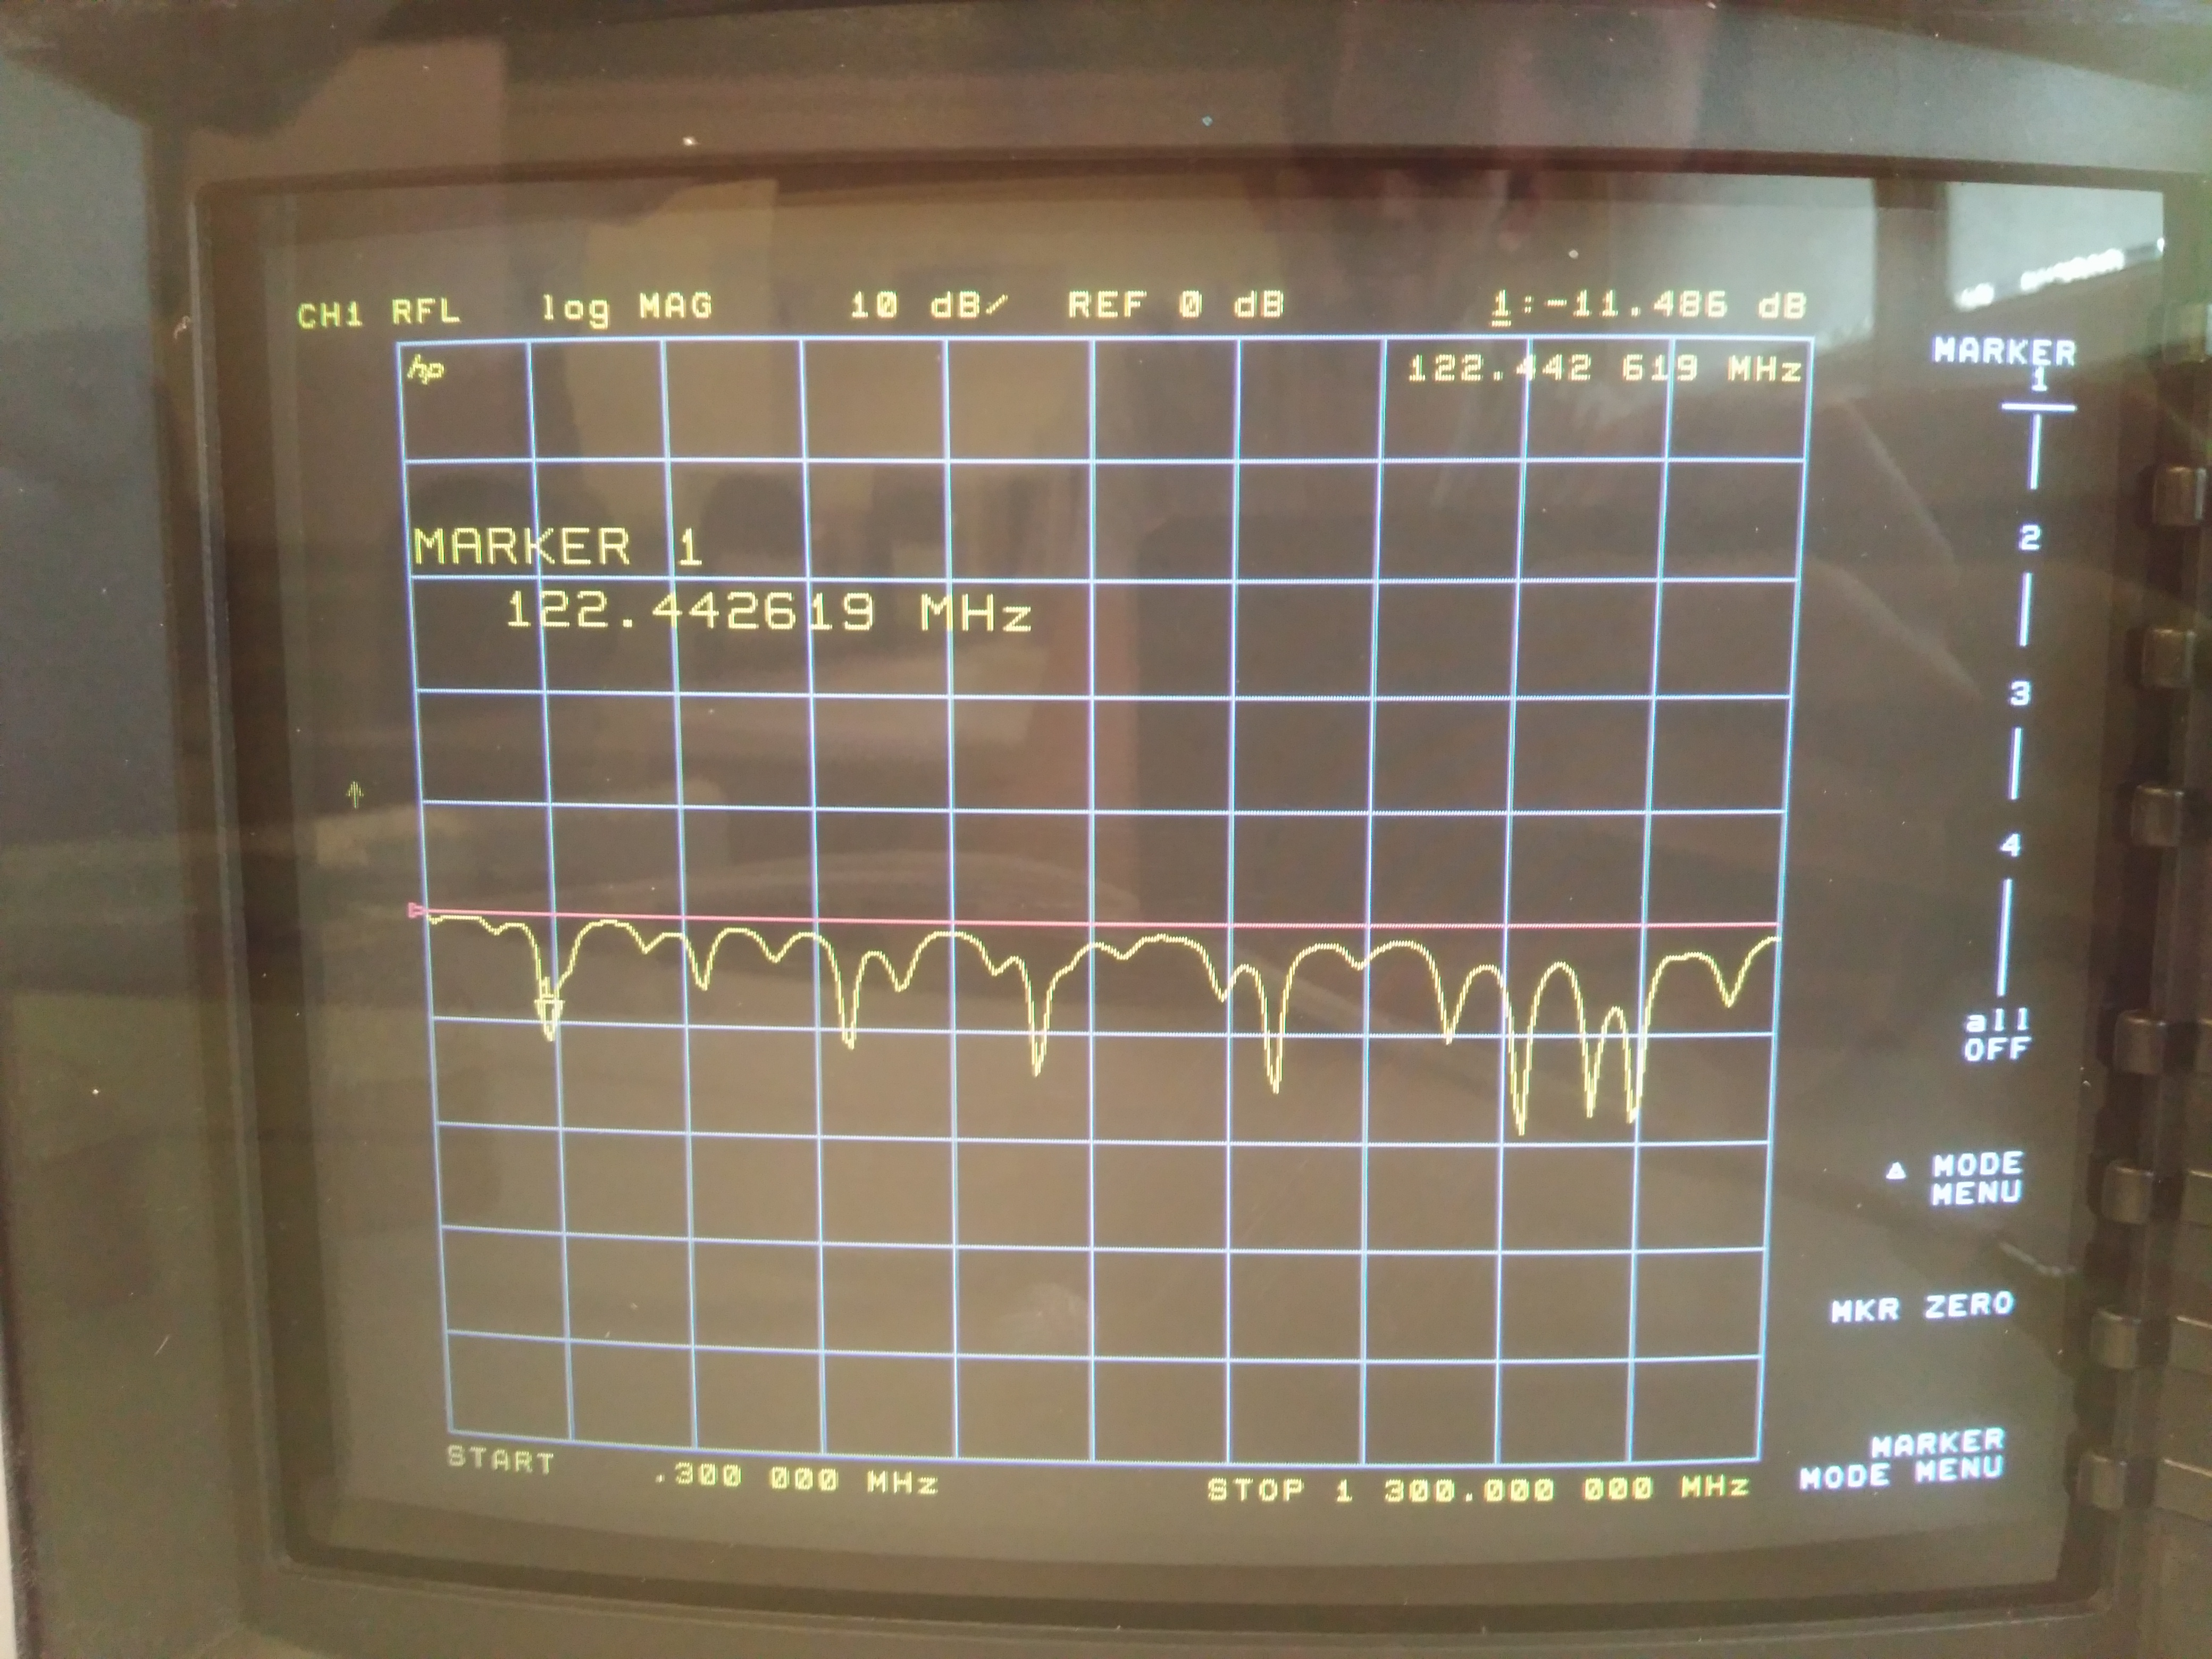
\includegraphics[width=\textwidth]{./images/Mesures/1reflx_broadband.jpg}
	\caption{|$\Gamma$| pel sistema connector-cable-balun-antena. 0.3 - 300 MHz }
	\label{1rflx}
\end{figure}
S'observa en la figura \ref{1rflx} que hi ha molts pics inversos. En aquests pics es on l'antena té un coeficient de reflexió baix, que és el que interessa. El primer d'aquests pics es troba sobre els 122MHz i és per al que hem dissenyat l'antena. La resta apareixen per efectes d'harmònics i altres fenòmens.
A continuació, a la figura \ref{2rflx} s'amplia a la zona que interessa estudiar.
\begin{figure}[H]
	\centering
	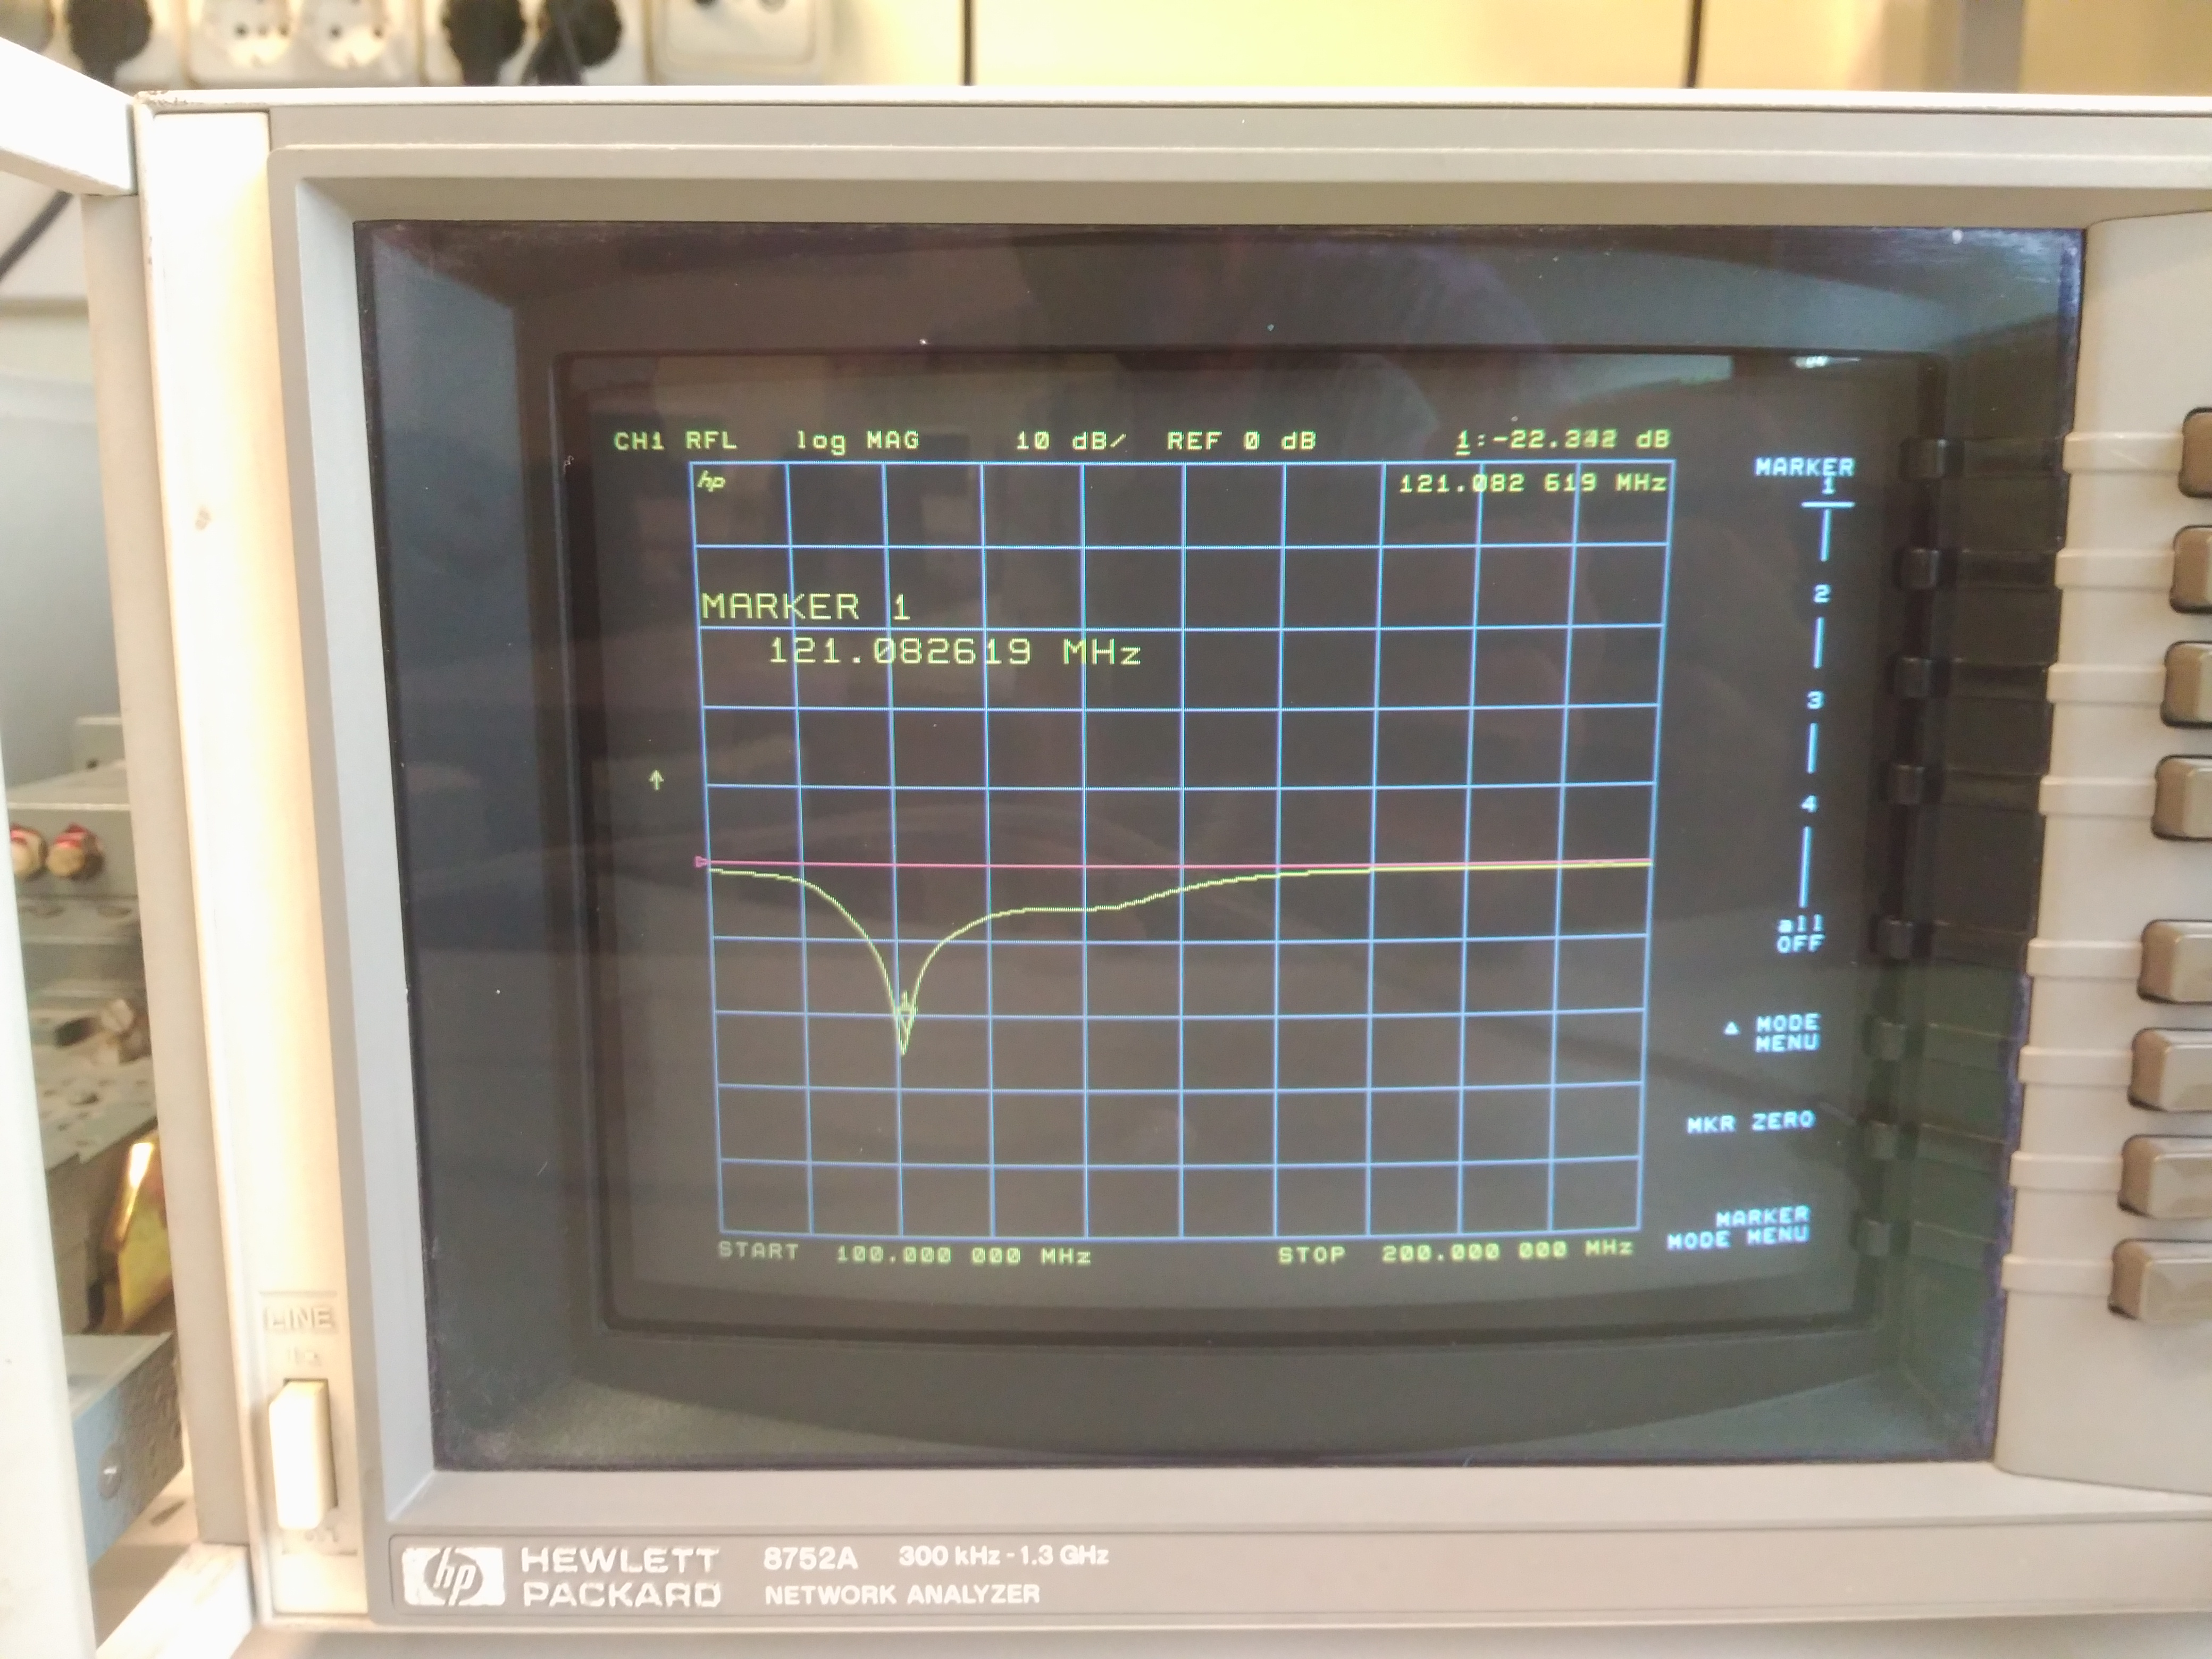
\includegraphics[width=\textwidth]{./images/Mesures/2relfx_narrowband.jpg}
	\caption{|$\Gamma$| pel sistema connector-cable-balun-antena. 100 - 300 MHz }
	\label{2rflx}
\end{figure}
D'aquí s'extreu que l'antena és òptima a 121.08MHz on presenta el següent resultat:
\begin{table}[H]
	\centering
	\begin{tabular}{lc}
		\toprule[3pt]
		\textbf{f}&\textbf{$\Gamma$}\\
		\midrule[1pt]
		121.08 & -20dB \\
		\bottomrule[2pt]
	\end{tabular}
	\caption{|$\Gamma$|}
	\label{gamma}
\end{table}
És considera que quan $\mid\Gamma\mid < -10dB$ l'antena està ben adaptada.
\subsection{Mesura del SWR}
També amb l'analitzador de xarxes, s'obté la mesura del SWR.
\begin{equation}
SWR =\frac{1+\mid\Gamma\mid}{1-\mid\Gamma\mid}
\end{equation}
\begin{figure}[H]
	\centering
	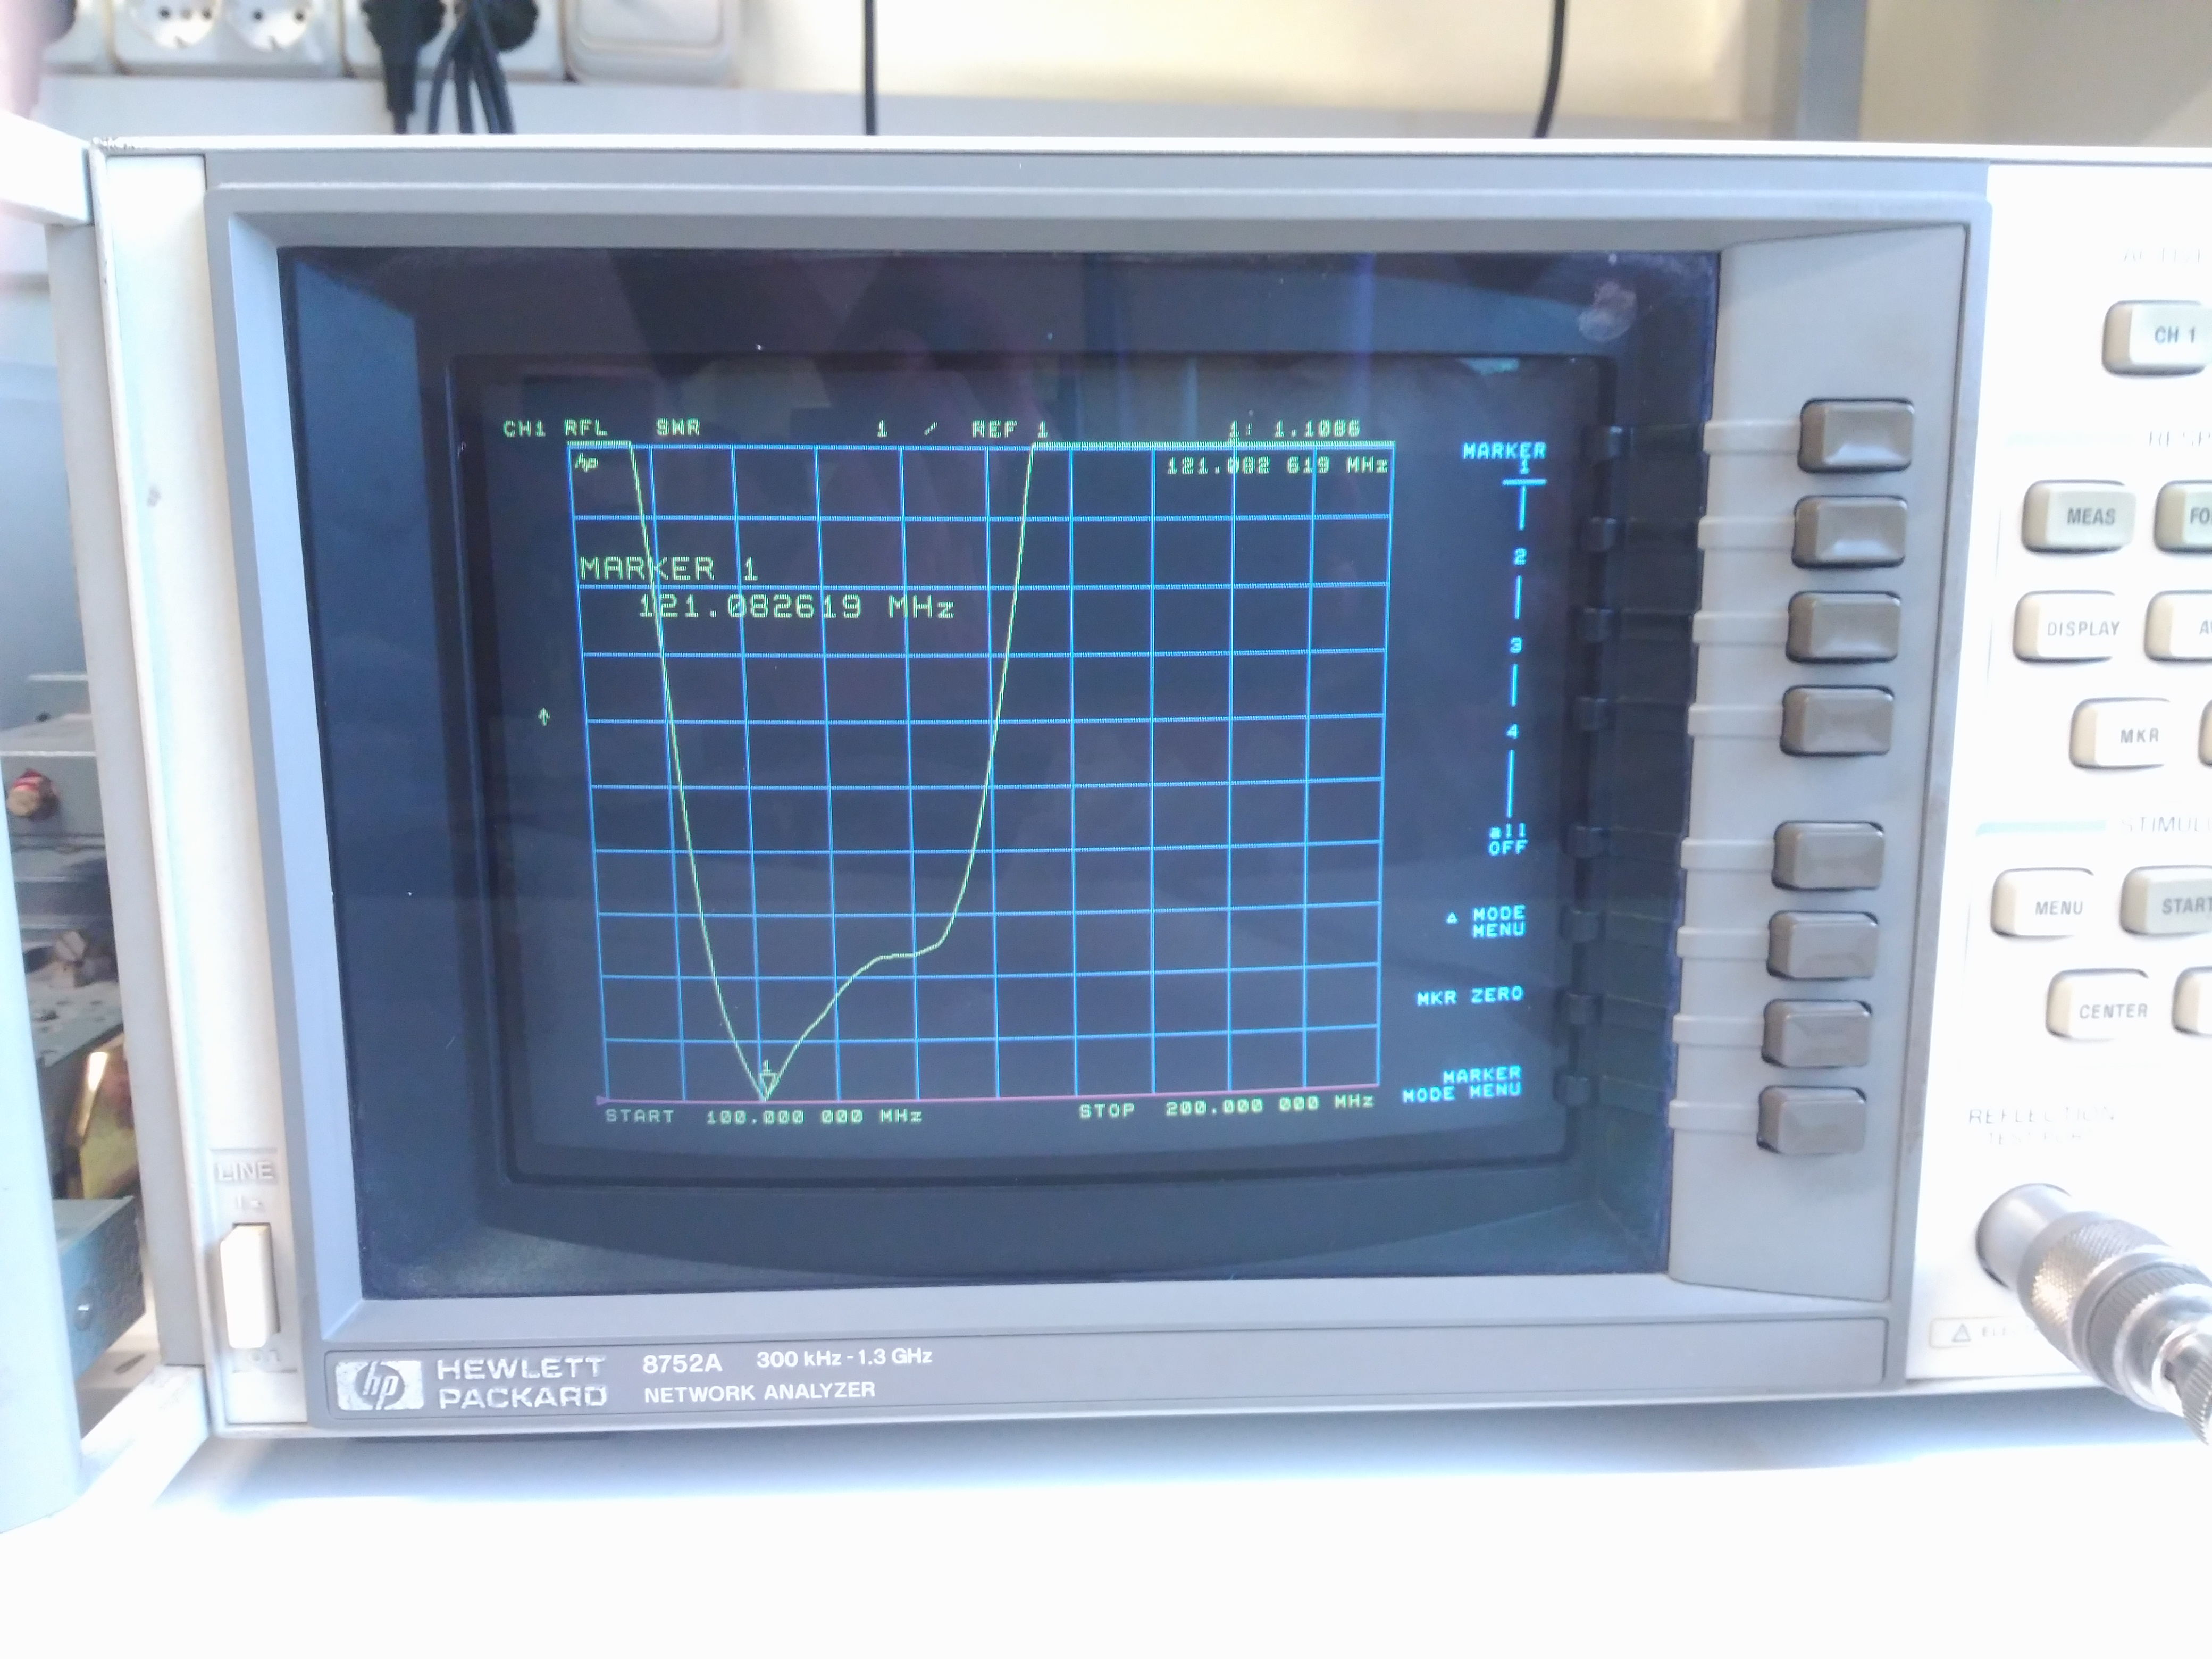
\includegraphics[width=\textwidth]{./images/Mesures/3swr.jpg}
	\caption{\textbf{SWR} pel sistema connector-cable-balun-antena. 100 - 200 MHz}
	\label{swr}
\end{figure}
S'obtè a la freqüència central un \textbf{SWR de 1.15}. Sempre i quan el SWR estigui per sota de 2, es considera que l'antena està ben adaptada. Sabent això s'ha mesurat el rang de freqüències operatives. 

Finalment s'ha vist que l'antena opera bé entre els \textbf{117MHz i els 127MHz}. Gairebé emplena tota la banda aeronàutica. Cal comentar que al tractar-se d'una antena dipol era d'esperar que el seu ample de banda sigui més limitat.
\subsection{Carta de Smith}
\begin{figure}[H]
	\centering
	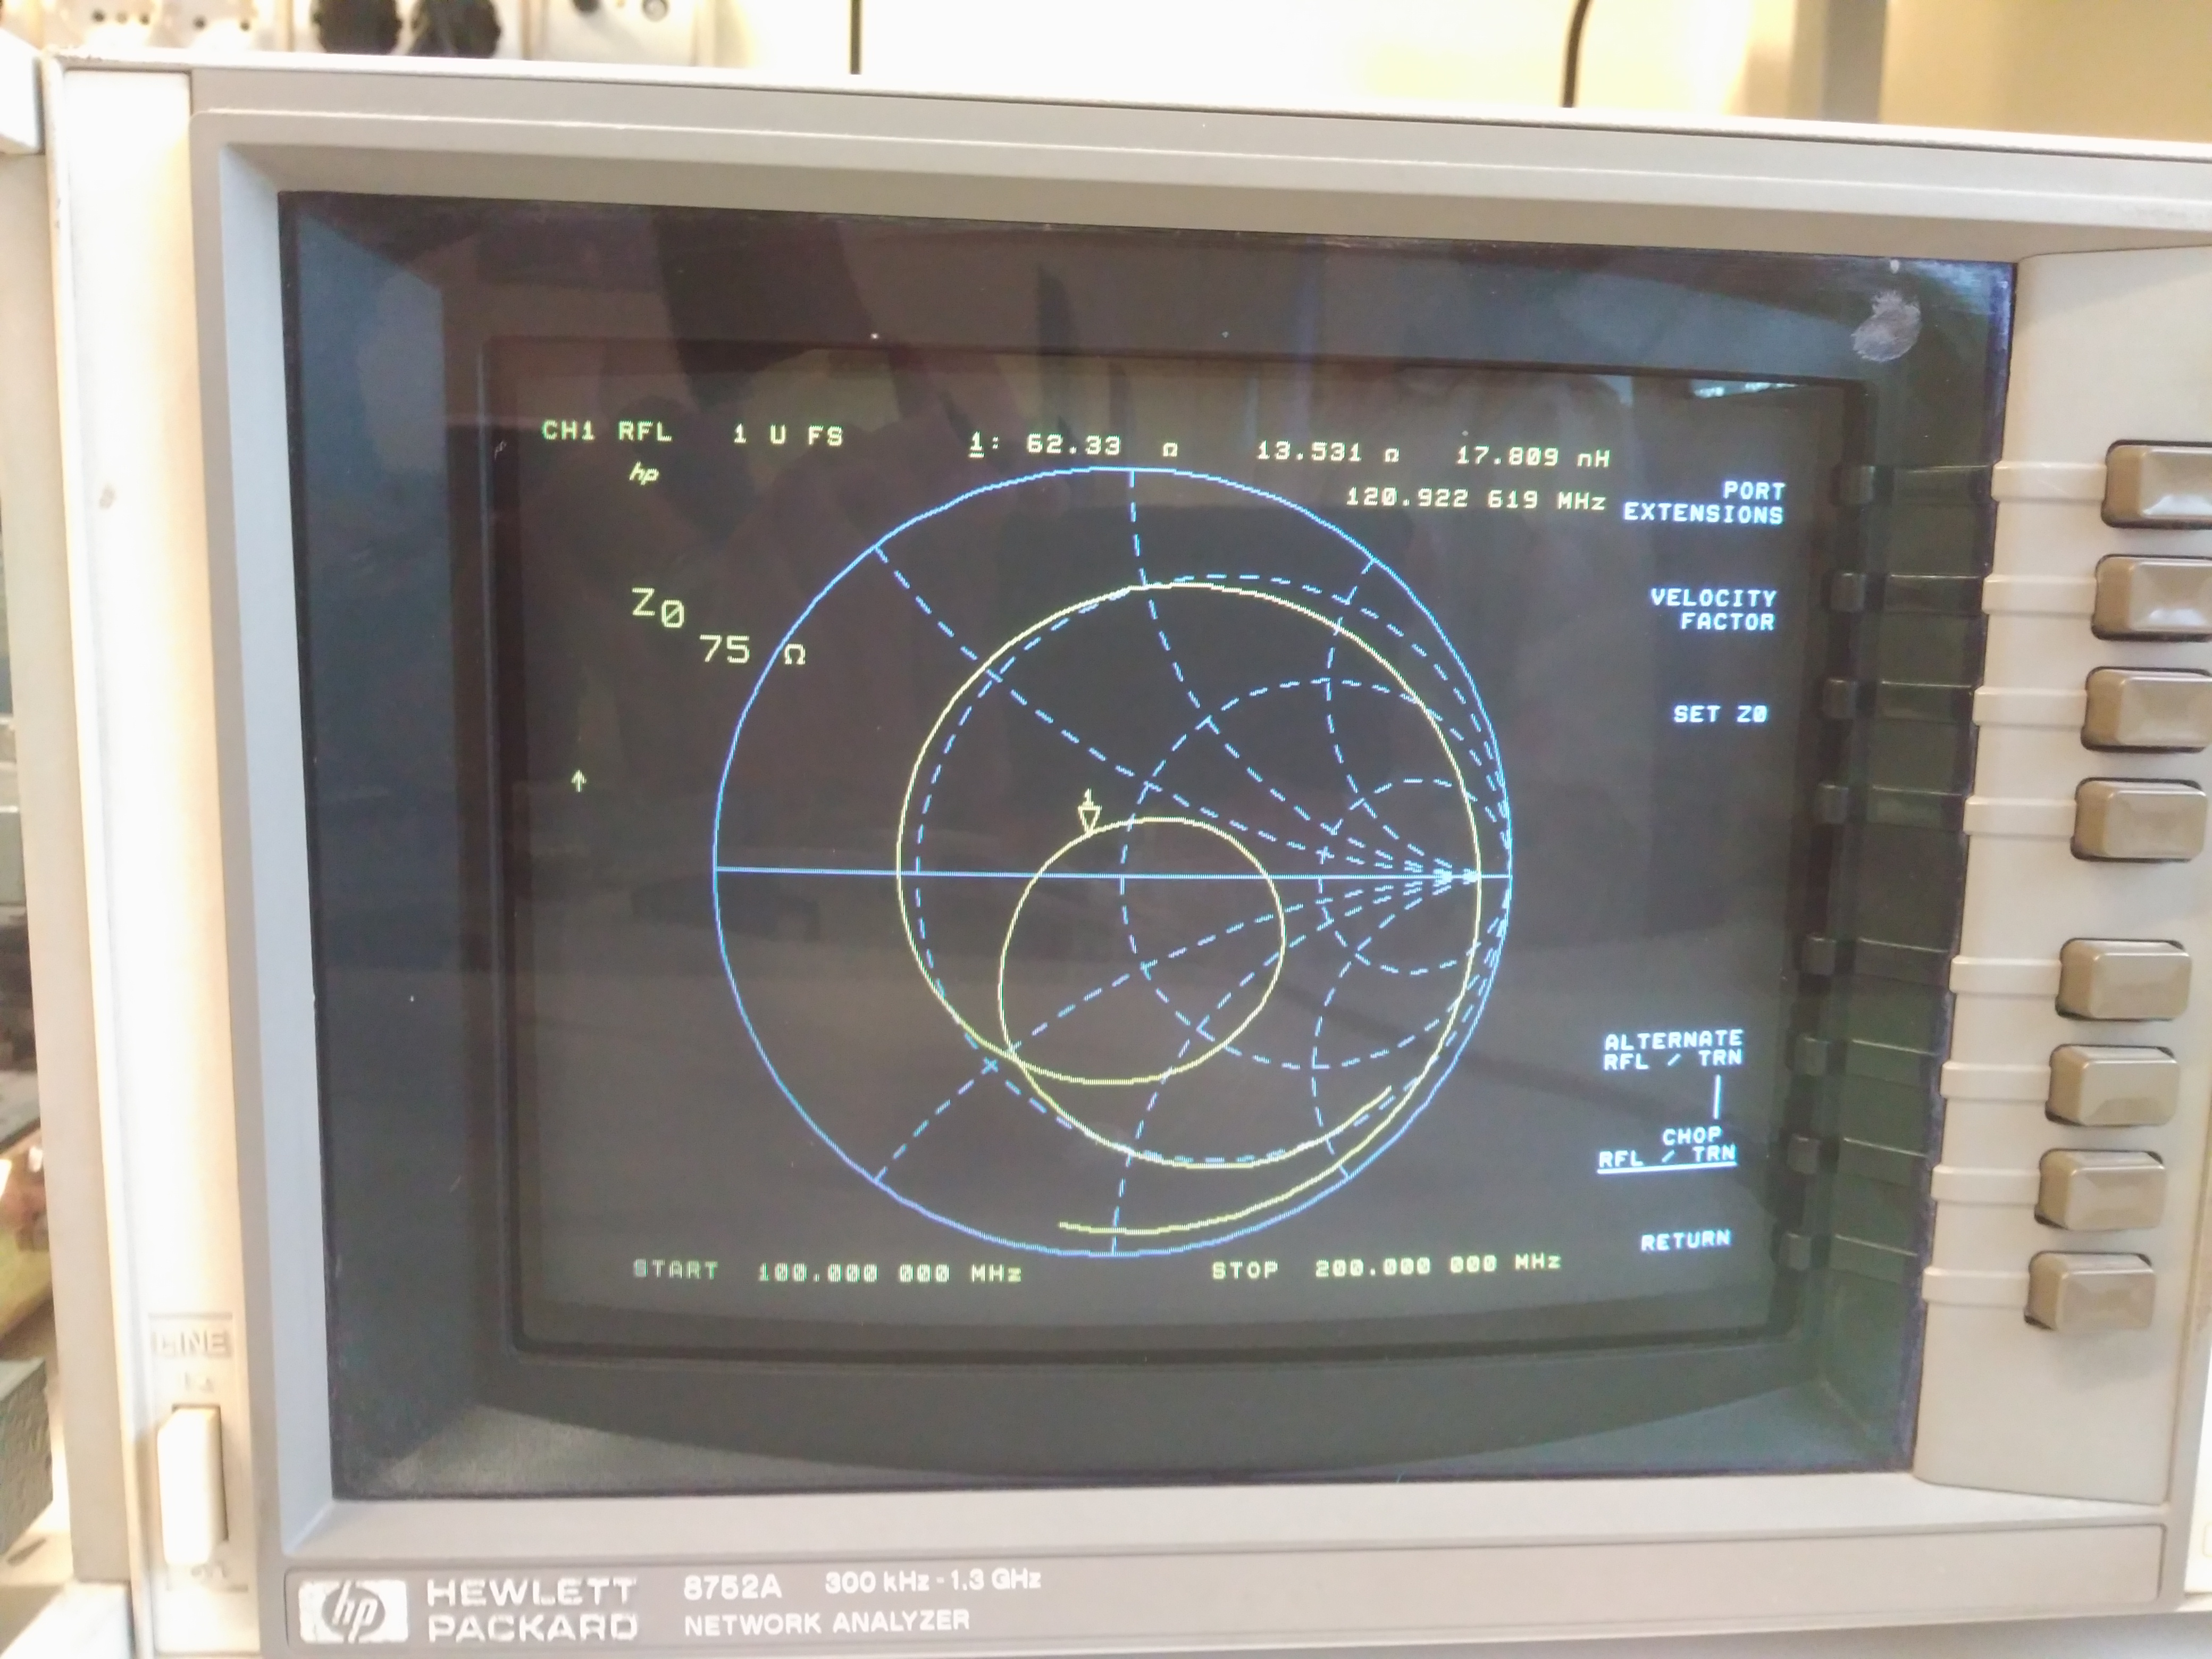
\includegraphics[width=\textwidth]{./images/Mesures/4smith.jpg}
	\caption{Carta de Smith}
	\label{smith}
\end{figure}
La carta de Smith també ha sigut obtinguda amb l'analitzador d'espectres configurat a 75 $\Omega$. Com es pot observar, el cursor està ben a prop del centre del cercle, ratificant així el fet que l'antena està ben adaptada.
La carta ens proporciona informació extra. Resulta que la impedància d'entrada en $\Omega$ del conjunt és:
\begin{equation}
Z = 62.3 + 17.8e-9	
\end{equation}
Observi's com la part imaginaria és gairebé nul·la, i com la real està molt a prop dels 73$\Omega$ teòrics calculats analíticament. S'ha de tindre en compte també que els 73 son únicament pel dipol, mentre que l'anterior és la de tot el sistema.
\subsection{Altres}
Finalment és va connectar l'antena a l'analitzador d'espectres. Amb un segon dipol situat a l'altra punta del laboratori es va emetre un to pur a la freqüència de 121MHz.
\begin{figure}[H]
	\centering
	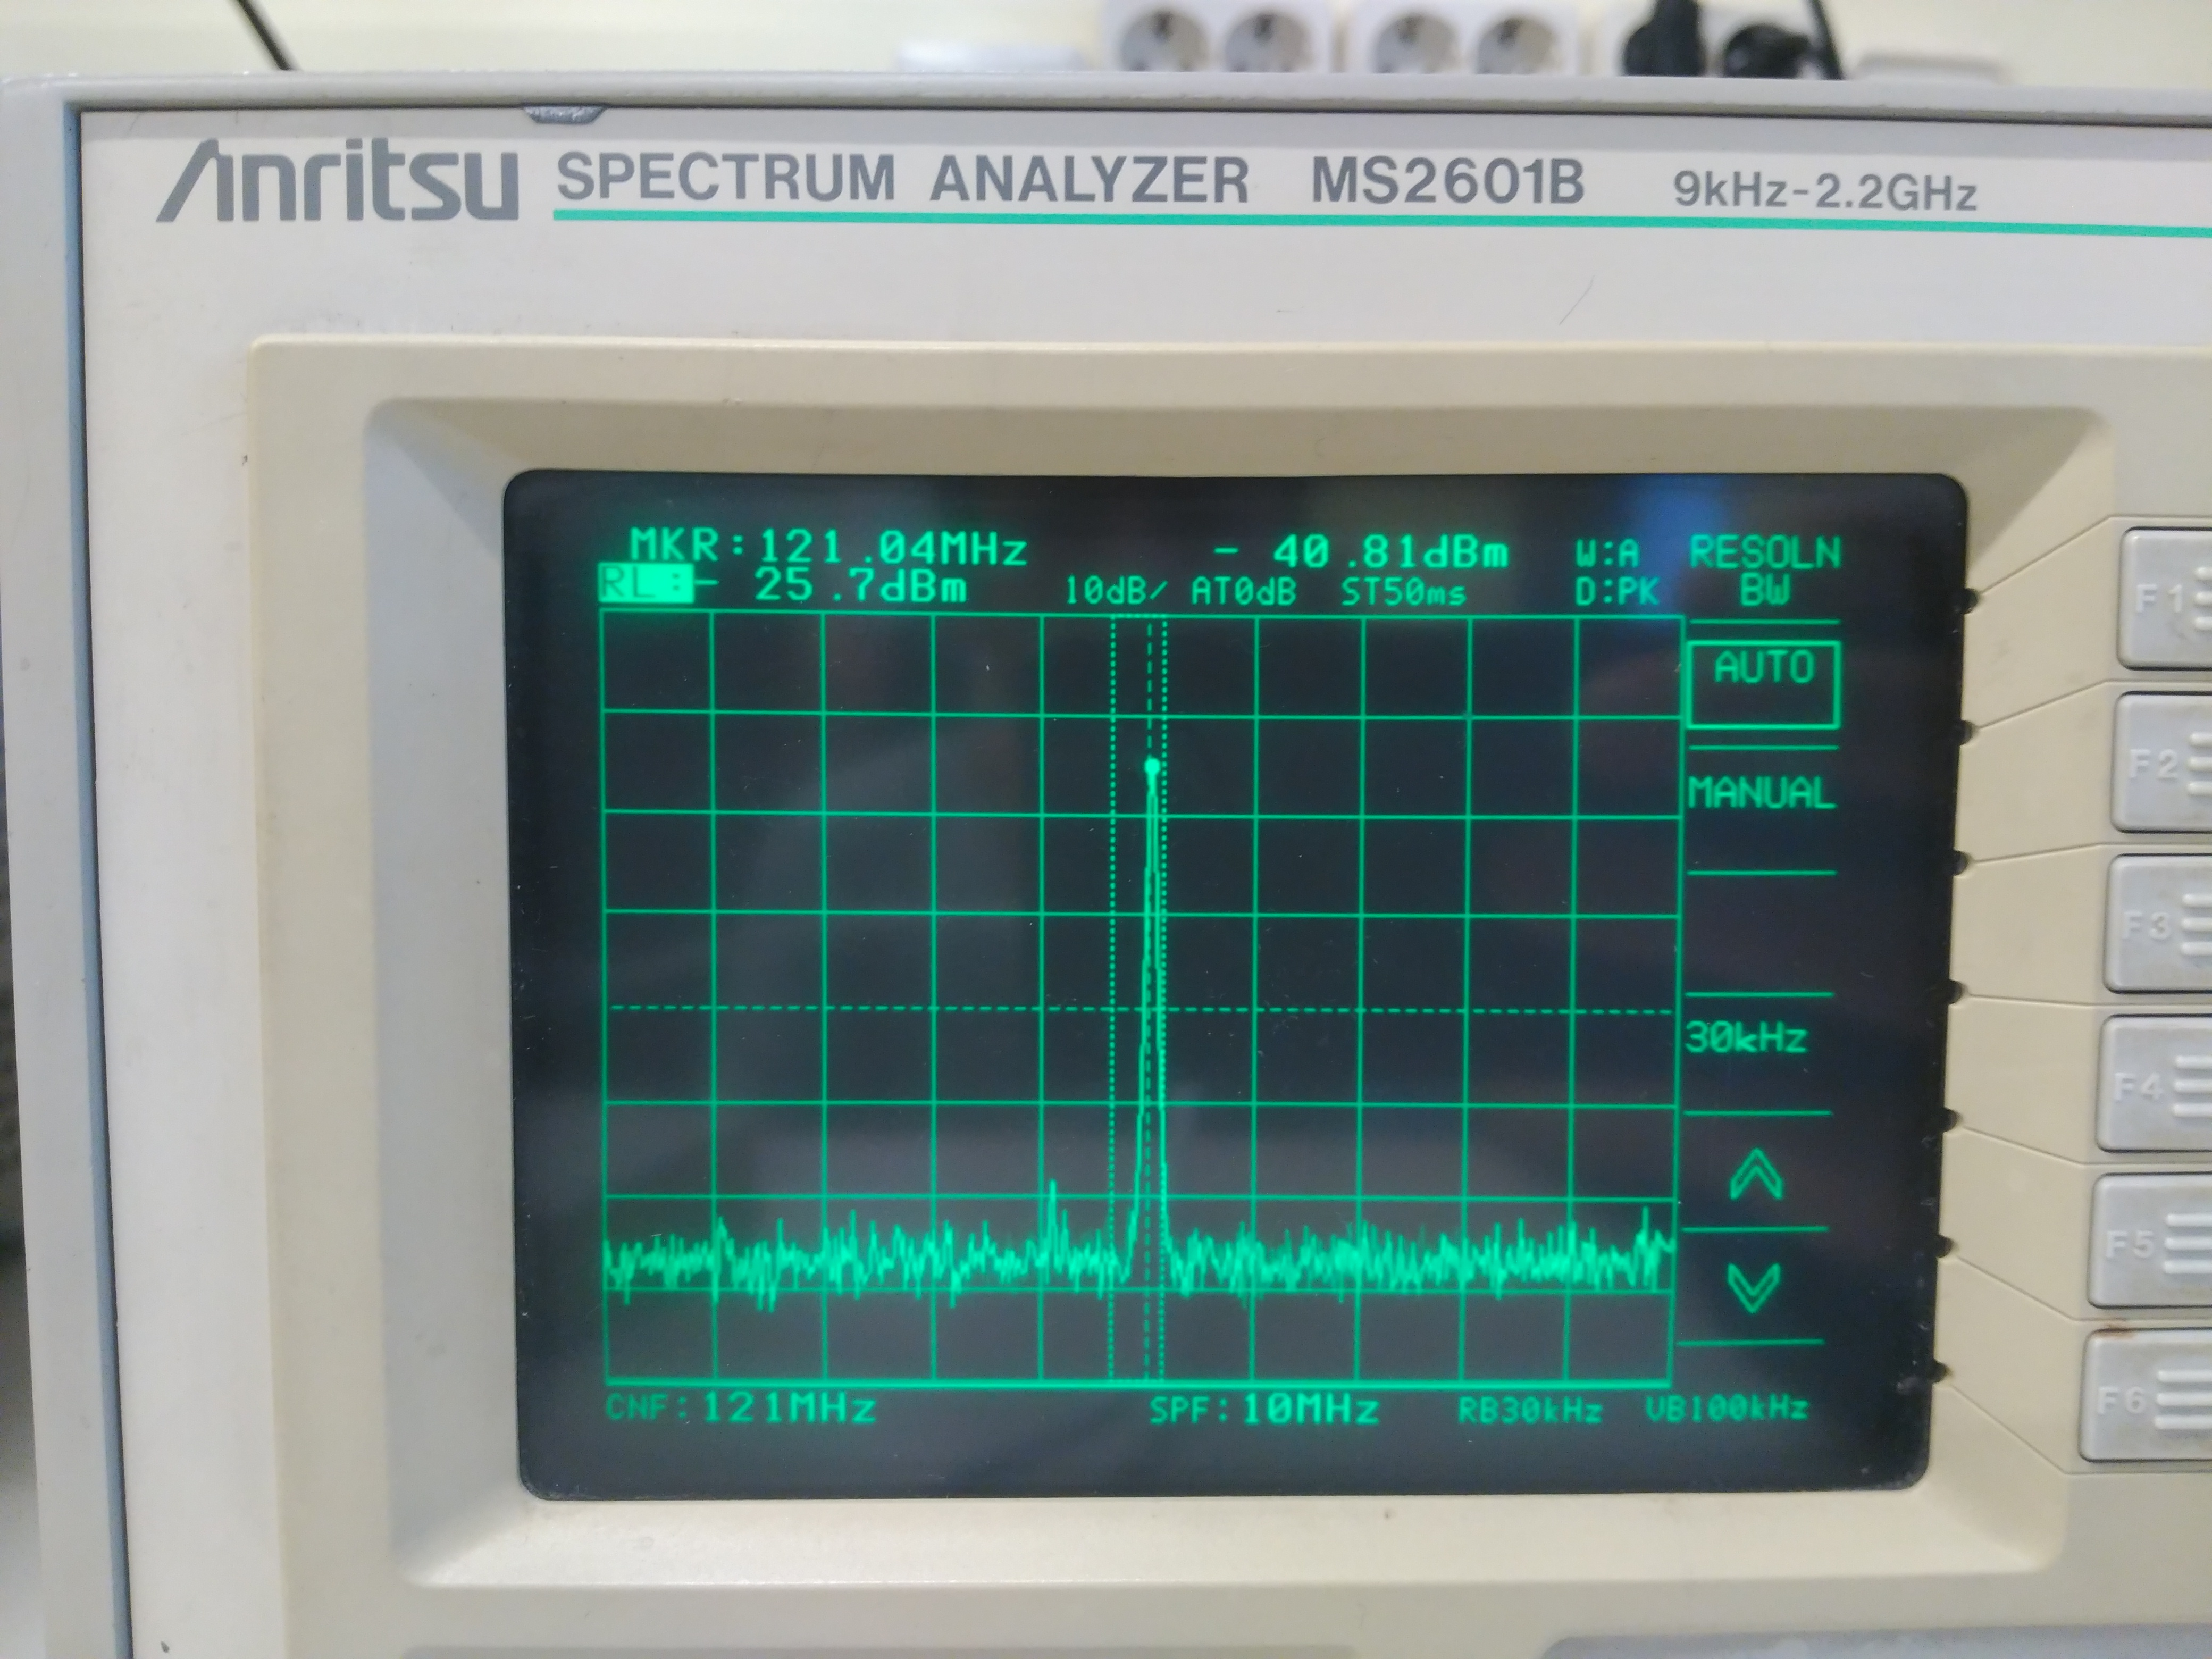
\includegraphics[width=\textwidth]{./images/Mesures/5recepcio.jpg}
	\caption{Comportament en recepció}
	\label{RX}
\end{figure}
Com es pot observar a la figura \ref{RX}, la senyal rebuda té un molt \textbf{bon SNR}. A més, la potència rebuda, segons va comentar el professor, era força alta comparativament. Si es disposés d'una càmera anecoica, amb aquest mateix experiment es podria determinar el diagrama de radiació de l'antena i comparar-ho amb el teòric calculat del 4NEC2.

A continuació, es va sintonitzar la radio des de el mateix analitzador d'espectres i aquesta es va rebre amb bona qualitat tot i estar fora del rang "òptim". 

Finalment, durant un segon experiment fet de forma autònoma (veure figura \ref{ExpAutonom}) pels integrants del grup, va ser possible escoltar a un avió aterrant a l'aeroport de Sabadell. Aquest es va fer connectant l'antena a una radio del tipus SDR que a la vegada estava connectada a l'ordinador.

\begin{figure}[H]
	\centering
	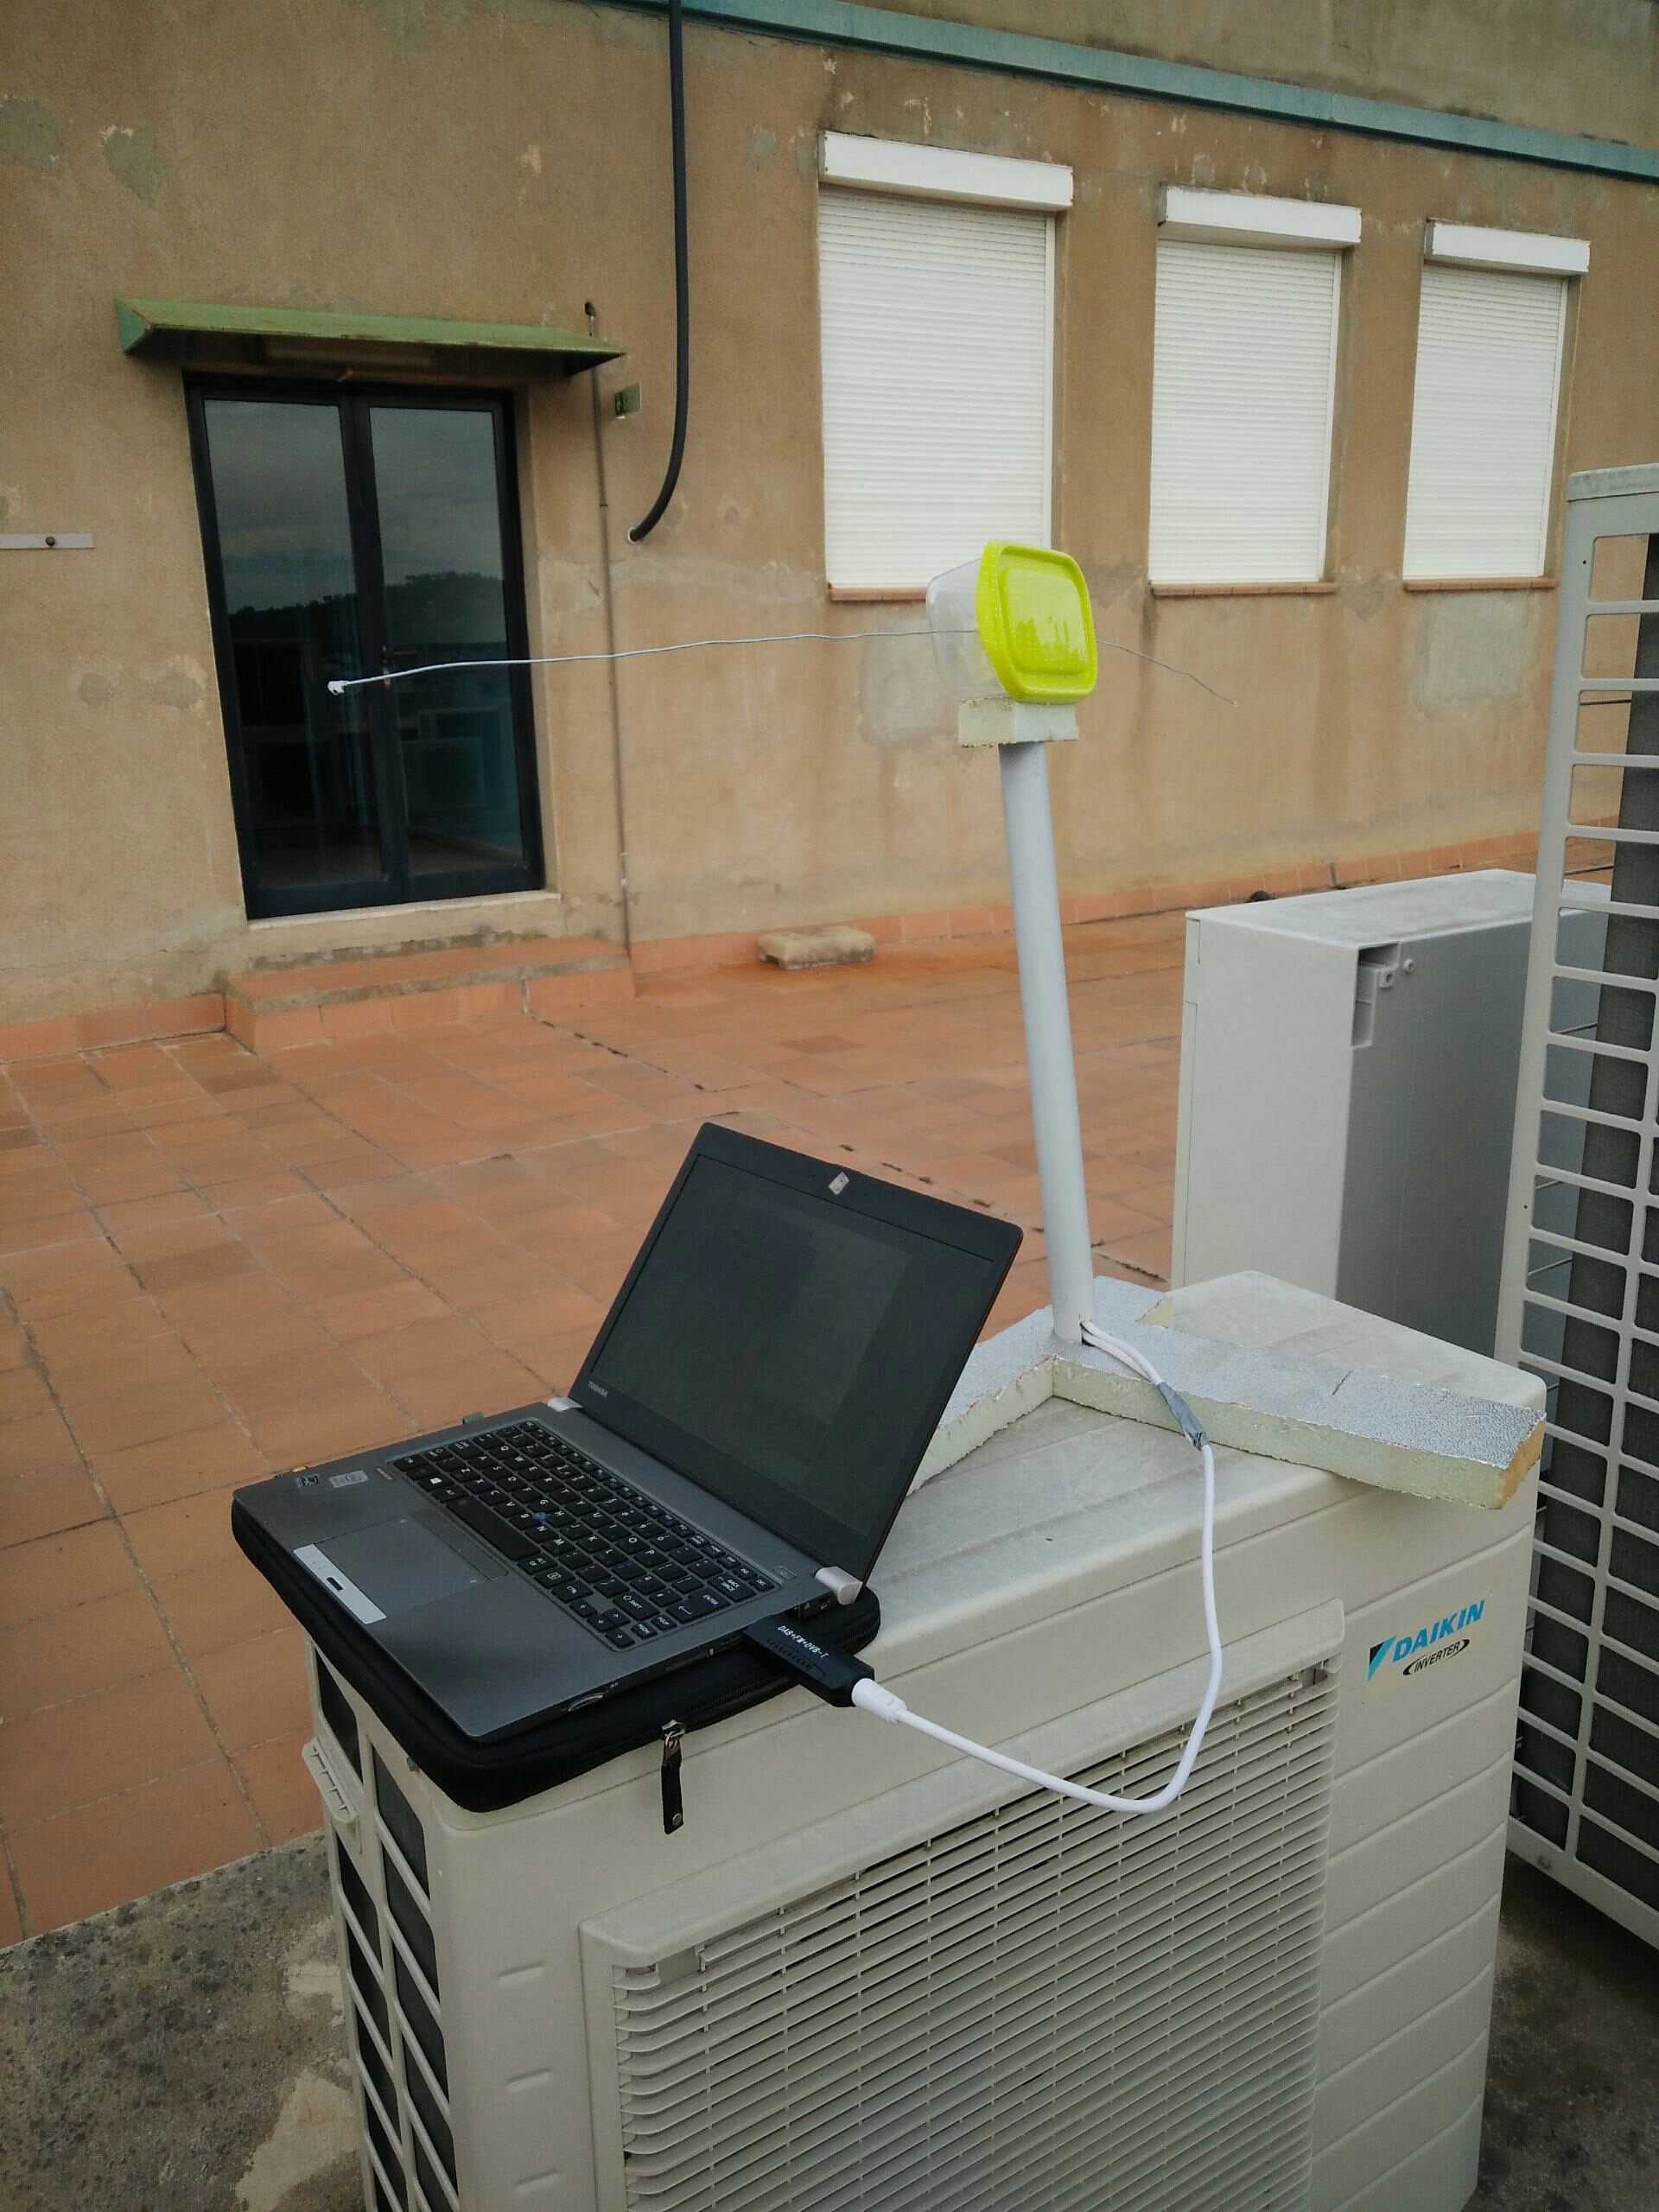
\includegraphics[width=0.5\textwidth]{./images/Mesures/Exp_autonom_1.jpg}
	\caption{Realització experiment autònom}
	\label{ExpAutonom}
\end{figure}
